% polyx.tex
\documentclass{article}
%\usepackage[boxed]{algorithm2e}
%\usepackage{comment}
%%% AMSMATH SUBS -- nonoptimal
%\newcommand{\eqref}[1]{(\ref{#1})}
%\newcommand{\operatorname}{\mbox}
%\newcommand{\operatornamewithlimits}{\mbox}
%\newcommand{\text}{\mbox}
%\newcommand{\argmin}{\mathop{arg\,min}}
%%%
%\newcommand{\argmin}{\operatornamewithlimits{arg\,min}}
%\usepackage{refcheck }
\usepackage{pdfpages}
\usepackage{longfbox}
\usepackage{latexsym}
\usepackage{amsthm}
\usepackage{amssymb}
\usepackage{amsmath}
\usepackage{graphicx}
\usepackage{tikz}
\usepackage{braket}
\usepackage{mathtools}
\usepackage{tensor}
\usepackage[compat=1.0.0]{tikz-feynman}
\usepackage{gensymb}
\usepackage[mathstyleoff]{breqn}
\usepackage{csquotes}
\usepackage{slashed}
\usepackage{empheq}

% Command "alignedbox{}{}" for a box within an align environment
% Source: http://www.latex-community.org/forum/viewtopic.php?f=46&t=8144
\newlength\dlf  % Define a new measure, dlf
\newcommand\alignedbox[2]{
	% Argument #1 = before & if there were no box (lhs)
	% Argument #2 = after & if there were no box (rhs)
	&  % Alignment sign of the line
	{
		\settowidth\dlf{$\displaystyle #1$}  
		% The width of \dlf is the width of the lhs, with a displaystyle font
		\addtolength\dlf{\fboxsep+\fboxrule}  
		% Add to it the distance to the box, and the width of the line of the box
		\hspace{-\dlf}  
		% Move everything dlf units to the left, so that & #1 #2 is aligned under #1 & #2
		\boxed{#1 #2}
		% Put a box around lhs and rhs
	}
}
\usetikzlibrary{babel}
\usetikzlibrary{positioning,arrows.meta}

\usepackage[spanish, activeacute]{babel} %Definir idioma español
\usepackage[utf8]{inputenc} %Codificacion utf-8
\usepackage{tkz-euclide}
\usepackage{esvect}
\usepackage{amsmath}
\DeclareMathOperator{\Tr}{Tr}
\usepackage{csquotes}
\usepackage{breqn}
\usepackage{hyperref}
\usepackage{caption}
\usepackage{gensymb}

\renewcommand\floatpagefraction{.95}
\renewcommand\topfraction{.95}
\renewcommand\bottomfraction{.95}
\renewcommand\textfraction{.05}
\renewcommand\floatsep{10pt}
\renewcommand\textfloatsep{10pt}
\renewcommand\intextsep{10pt}
\renewcommand{\baselinestretch}{1.5} 

% These four commands are to fix equation numbering
%\makeatletter
%\renewcommand\theequation{\thesection.\arabic{equation}}
%\@addtoreset{equation}{section}
%\makeatother
%***************************%
\iffalse
% STRONG margin Manipulation
\setlength{\topmargin}{7mm}
\setlength{\topmargin}{-.5in}
\setlength{\oddsidemargin}{-.3in}
\setlength{\evensidemargin}{-.3in}
\setlength{\textwidth}{1.5\textwidth} % Make are margins wider
\setlength{\textheight}{1.15\textheight}
%\setlength{\oddsidemargin}{0.1\oddsidemargin}
%\setlength{\evensidemargin}{0.1\evensidemargin}
\fi

\iffalse
% MODERATE margin Manipulation
%\setlength{\topmargin}{7mm} % Is top margin useful to manipulate?
%\setlength{\topmargin}{-.5in}
%\setlength{\oddsidemargin}{-.1in}
%\setlength{\evensidemargin}{-.1in}
\setlength{\textwidth}{1.1\textwidth} % Make are margins wider
\setlength{\textheight}{1.15\textheight}
\fi
%%% ad-hoc spacing commands


\iffalse
% NEW (milder) margin Manipulation
%\setlength{\topmargin}{7mm} % Is top margin useful to manipulate?
%\setlength{\topmargin}{-.5in}
%\setlength{\oddsidemargin}{-.1in}
%\setlength{\evensidemargin}{-.1in}
\setlength{\textwidth}{1.05\textwidth} % Make are margins wider
\setlength{\textheight}{1.15\textheight}
\fi
%%% ad-hoc spacing commands
\newcommand{\vmina}{\vspace{-.1in}}
\newcommand{\vminb}{\vspace{-.03in}}


%\iffalse
\theoremstyle{plain}
\newtheorem{theorem}{Theorem}[section]
\newtheorem{lemma}[theorem]{Lemma}
\newtheorem{corollary}[theorem]{Corollary}
\theoremstyle{definition}
\newtheorem{definition}[theorem]{Definition}
\newtheorem{italg}[theorem]{Algorithm}
\newtheorem{itexamp}[theorem]{Example}
%\fi

\newtheorem{myclaim}{Claim}



\newcommand\myset[2]{ \left\{ {#1} \,:\, {#2} \right\} }
\newcommand\Binsum[2]{ { {#1} \choose \leq {#2} } }
\newcommand{\fset}{{\cal U}}
\newcommand\marcom[1]{\marginpar{{\bf\small{#1}}}}


\newcommand{\bu}{\mathbf u}
\newcommand{\bv}{\mathbf v}
\newcommand{\bx}{\mathbf x}
\newcommand{\bw}{\mathbf w}
\newcommand{\by}{\mathbf y}
\newcommand{\bzero}{\mathbf 0}
\newcommand{\bh}{\mathbf h}

\newcommand{\predprob}{ {\rho} }
%\newcommand{\predexp}{ {\phi} }
\newcommand{\loss}{ {L} }
\newcommand{\expt}{ {\cal E} }

\newcommand{\sumn}{{\sum_{i=1}^n}}
\newcommand{\sumtl}{{\sum_{t=1}^{\ell}}}
\newcommand{\sumsts}{{\sum_{t=s}^{s'}}}

\newcommand{\res}{{\rho}}


\newcommand{\xt}{ {{\bf x}_t}}
\newcommand{\xti}{{x_{t,i}}}
\newcommand{\xtj}{{x_{t,j}}}

\newcommand{\ds}{{Z}}
\newcommand{\dsln}{{Z_{\ln}}}
\newcommand{\dsid}{{Z_{\mbox{id}}}}
\newcommand{\dsm}{{\bz}}
\newcommand{\dsmc}{{z}}


%\newcommand{\wt}{ \mbox{\boldmath$w$}_t }
%\newcommand{\wts}{ \mbox{\boldmath$w$}_{t+1} }
\newcommand{\wt}{\mathbf w_t }
\newcommand{\wts}{\mathbf w_t}

\iffalse
\newcommand{\wti}{w_{t,i}}
\newcommand{\wtsi}{w_{t+1,i}}
\newcommand{\wtj}{w_{t,j}}
\newcommand{\wtsj}{w_{t+1,j}}
\fi

\newcommand{\vt}{\mathbf v_t }
\newcommand{\vts}{\mathbf v_{t+1}}
\newcommand{\vti}{v_{t,i}}
\newcommand{\vtsi}{v_{t+1,i}}
\newcommand{\vtj}{v_{t,j}}
\newcommand{\vtsj}{v_{t+1,j}}

\newcommand{\ut}{\mathbf u_t}
\newcommand{\uts}{\mathbf u_{t+1}}
\newcommand{\uti}{u_{t,i}}
\newcommand{\utsi}{u_{t+1,i}}
\newcommand{\utsj}{u_{t+1,j}}

\newcommand{\sumin}{{\sum_{i=1}^n}}
\newcommand{\sumim}{{\sum_{i=1}^m}}
\newcommand{\sumjm}{{\sum_{j=1}^m}}
\newcommand{\sumjn}{{\sum_{j=1}^n}}
\newcommand{\sumit}{{\sum_{i=1}^t}}
\newcommand{\sumjt}{{\sum_{j=1}^t}}
\newcommand{\sumik}{{\sum_{i=1}^k}}
\newcommand{\norm}[1]{{\|{#1}\|}}


\newcommand{\lat}{{L_{A,t}}}
\newcommand{\lut}{{L_{\bu,t}}}
\newcommand{\lit}{{L_{i,t}}}
\newcommand{\unif}{{\frac{1}{n}}}

\newcommand{\aksched}{{<([t_0,t_1),\bu_0),([t_1,t_2),\bu_1),\ldots,
		([t_{k},t_{k+1}),\bu_k)>}}
\newcommand{\flut}{{L(S,\!<\!\bu\!>\!)}}

%\newcommand{\equref}[1]{(\ref{#1})}
\newcommand{\pred}{ {\hat{y} }}
\newcommand{\predt}{ {\hat{y}_t} }
\newcommand{\predtqg}{ {\hat{\by}^{i}_t(\gparm)} }
\newcommand{\predjqg}{ {\hat{\by}^{i}_j(\gparm)} }


\newcommand{\outc}{ {y} }
\newcommand{\outct}{ {y_t} }
\newcommand{\epredt}{ {x_{t,i}} }
\newcommand{\lpt}{ {\cal P} }
\newcommand{\Lu}{{\hat{L}}}
\newcommand{\lu}{{\hat{\ell}}}
\newcommand{\ku}{{\hat{k}}}
\newcommand{\lossofalgonseq}{{L(S,A)}}
\newcommand\floor[1]{{\left\lfloor {#1} \right\rfloor}}
\newcommand\ceil[1]{{\left\lceil {#1} \right\rceil}}
%\newcommand{\implies}{{\Rightarrow}}
%\newcommand{\mapsto}{{\Rightarrow}}

\newcommand{\binomg}[2]{{\binom{#1}{#2}}_{\Gamma}}
\newcommand{\aprior}{{f(p)}}
%\newcommand{\ws}[2]{{\omega_{{#1},{#2}}}}
%\newcommand{\wstk}{{\ws{t}{k}}}
\newcommand{\ssh}{{\alpha}}
\newcommand{\sss}[2]{{\alpha_{{#1},{#2}}}}
\newcommand{\sstk}{{\sss{t}{k}}}
\newcommand{\intersex}{{\bigcap}}
%\newcommand{\cclass}{{\cal}}

%\newcommand{\proj}[3]{{P_{{#1},{#2}}({#3})}}
\newcommand{\projeu}[2]{{{\cal P}_{{#1}}({#2})}}
\newcommand{\proj}[2]{{{\cal P}_{{#2}}({#1})}}



% \input{mjhbibmacs}
\newcommand{\coverbook}{***}
\newcommand{\decgenboost}{{fs-dgolab-95}}
\newcommand{\dotprodpaper}{w-pdefw-97}
\newcommand{\vovktrack}{b-dsps-97}
\newcommand{\specialist}{fssw-se-97}
\newcommand{\trackii}{h-tbet-97}
\newcommand{\yoramport}{s-trcpsa-97}
\newcommand{\diskidle}{hls-ddstmc-96}
\newcommand{\mtstrack}{bb-olmts-97}
\newcommand{\newvovk}{v-gpea-95}
\newcommand{\tracklong}{herbster98tracking}
\newcommand{\hkw}{hkw-spisglf-98}
\newcommand{\eg}{kw-avegulp-97}
\newcommand{\wm}{lw-wma-94}
\newcommand{\experts}{cfhhsw-huea-97}
\newcommand{\gd}{clw-wqlbop-96}
\newcommand{\hadapaper}{kw-pavwlvl-95}
\newcommand{\agnostic}{kss-teal-94}
\newcommand{\csiszaraxiom}{c-wylmeaa-91}

\newcommand{\kacz}{k***}
\newcommand{\mycapp}{***}
\newcommand{\mycuni}{***}
\newcommand{\kullbook}{***}
%\newcommand{\regressionbndpaps}{***}
\newcommand{\nellobook}{CriSha00}
\newcommand{\perceptron}{r-ppmisob-58}
\newcommand{\roseperc}{r-ppmisob-58}
\newcommand{\vonneumproj}{neumanproj}
\newcommand{\bbproj}{Bauschke:1996:PAS}
\newcommand{\fabmyceil}{fm-alt-91}
\newcommand{\novikoff}{n-ocpp-63}
\newcommand{\kernperc}{fs-lmcpa-99}
\newcommand{\kerntron}{fcc-kafslps-98}
\newcommand{\romma}{ll-romma-01}
\newcommand{\smotron}{Platt99}
\newcommand{\genlarmar}{sc-frmd-99}
\newcommand{\trackdisj}{aw-tbd-98}
\newcommand{\derand}{b-dsps-97}
\newcommand{\metrical}{bb-olmtsp-00}
\newcommand{\shifttheory}{\wm,\tracklong,\trackdisj,\derand,\metrical,\trakregr}
\newcommand{\trakregr}{hw-tbr-98}
\newcommand{\rkhsaron}{a-trk-50}
\newcommand{\vapchertpr}{vc-tpr-74}
\newcommand{\boguyvap}{bgv-taomc-92}
\newcommand{\origmetpot}{abr-thpfmprl-64}
\newcommand{\vovkkern}{sgv-rrladv-98}
\newcommand{\nickthesis}{l-mbllla-89}
\newcommand{\winnow}{l-liaanla-88}
\newcommand{\wcsingle}{hkw-rlbsn-01}
\newcommand{\Mycielski}{m-lalo-88}
\newcommand{\vovk}{v-as-90}
\newcommand{\smolatalk}{smolatalk00}
\newcommand{\rudinreplex}{IB-E883108}
\newcommand{\azoury}{aw-rlbodeefd-99}
\newcommand{\selfconfident}{acbg-ascolla-2003}
\newcommand{\vovkcompete}{vovk99competitive}
\newcommand{\vovkregression}{\vovkcompete}
%\newcommand{\vovkregression}{nips-10:Vovk:1998}
\newcommand{\avgexpert}{kivinen99averaging}
\newcommand{\jaaktrack}{NIPS2003_LT04}
% \newcommand{\ridge}{v-colr-97}
\newcommand{\foster}{f-pitwc-97}
\newcommand{\hoeff}{h-pisbrv-63}
\newcommand{\jyrklms}{nips02-AA33}
\newcommand{\fastkern}{h-lamofek-01}
\iffalse
\newcommand{\gproffline}{n-rcgpp-98,Williams1996Gaussian,gibbs-eff97,smola00sparse}
\newcommand{\gpronline}{nc:Csato+Opper:2002,NIPS2003_AA15}
\fi
\newcommand{\gproffline}{Williams1996Gaussian,gibbs-eff97}
\newcommand{\gpronline}{nc:Csato+Opper:2002,NIPS2003_AA15}

\newcommand{\ibcoverview}{TraubWerschulz98}
\newcommand{\mcmcsurvey}{mach:Andrieu+Freitas+Doucet:2003}
\newcommand{\approxperm}{jerrum01polynomialtime}
\newcommand{\mcmcvol}{dfr-rptaavcb-91}
\newcommand{\biasedcoin}{f-pbsawob-96}
\newcommand{\realcomplex}{bcss-cr-98}
\newcommand{\yapbook}{y-fpaa-00}
\newcommand{\pansurvey}{pan97solving}
\newcommand{\massicvxkern}{mp-lkfr-04}

%\newcommand{\cs}{{\Gamma}}
%\newcommand{\csp}{{\gamma}}
%\newcommand{\csa}{{\cs_{\csp}}}



\newcommand{\into}{{\rightarrow}}
\newcommand{\df}{d}
\newcommand{\simplex}{{\Delta}}
\newcommand{\dmu}{d\mu}
\newcommand{\ft}{{f_{t}}}
\newcommand{\fts}{{f_{t+1}}}
\newcommand{\ff}{{f^*}}
\newcommand{\Kxt}{K(\xt,\cdot)}
\newcommand{\dre}{{d_{\mbox{re}}}}
\newcommand{\dsq}{{d_{\mbox{sq}}}}

\newcommand{\bwt}{\bw_t}
\newcommand{\bwts}{\bw_{t+1}}
\newcommand{\bwls}{\bw_{\ell+1}}




\newcommand{\dop}[1]{{\langle{#1}\rangle}}
\newcommand{\dotp}[2]{{\langle{#1,#2}\rangle}}
\newcommand{\sign}{\operatorname{sign}}
\newcommand{\rent}{\operatorname{RE}}
\newcommand{\hispace}{{\cal H}}
\newcommand{\prehispace}{H}
\newcommand{\hispacegp}{{\cal H}_\gparm}
\newcommand{\prehispacegp}{H_{\gparm}}
\newcommand{\exspace}{{\cal X}}
\newcommand{\kf}{k}
\newcommand{\kgp}{k_{\gparm}}
\newcommand{\kgpt}{k_{\gparm}(x_t,\cdot)}

\newcommand{\seq}{\{(\bx_1,y_1),\ldots,(\bx_{\ell},y_{\ell})\}}
\newcommand{\sequ}{\{(\bx_1,y_1),\ldots\}}
\newcommand{\aseq}{\{(x_1,y_1),\ldots,(x_{\ell},y_{\ell})\}}
\newcommand{\kseq}{\{(K(x_1,\cdot),y_1),\ldots,(K(x_{\ell},\cdot),y_{\ell})\}}
\newcommand{\ssequ}{\{(x_1,y_1),\ldots\}}
\newcommand{\asequ}{\{(K(x_1,\cdot),y_1),\ldots\}}
\newcommand{\fseq}{\{\fset_1,\ldots,\fset_{\ell}\}}
\newcommand{\fsequ}{\{\fset_1,\ldots\}}
\newcommand{\lhs}{\operatorname{lhs}}
\newcommand{\rhs}{\operatorname{rhs}}
\newcommand{\lhsa}[1]{\operatorname{lhs}_{\{{#1}\}}}
\newcommand{\rhsa}[1]{\operatorname{rhs}_{\{{#1}\}}}
\newcommand{\gsa}[1]{\operatorname{gs}_{\{{#1}\}}}
%\newcommand{\argmin}{\operatornamewithlimits{arg\,min}}
\newcommand{\indi}{{\chi}}

\newcommand{\lms}{{\sc lms }}
\newcommand{\lmsns}{{\sc lms}}
\newcommand{\fuse}{{\sc k-lms-net }}
\newcommand{\fusens}{{\sc k-lms-net}}
\newcommand{\ewalg}{{\sc clipped exponential weights }}
\newcommand{\emewalg}{{\em exponential weights }}
\newcommand{\mcmc}{{\sc mcmc }}
\newcommand{\mcmcns}{{\sc mcmc}}
\newcommand{\onehalf}{\frac{1}{2}}
\newcommand{\parm}{\alpha}
\newcommand{\dparm}{d\parm}
\newcommand{\yhat}{\hat{y}}
\newcommand{\oner}{\frac{1}{r}}
\newcommand{\onez}{\frac{1}{z}}
%\newcommand{\onec}{\frac{1}{c}}
\newcommand{\oneeps}{\frac{1}{\epsilon}}
\newcommand{\epsi}{\epsilon}

\newcommand{\absepsa}[1]{{\overset{a}{\approx}}_{#1}}
\newcommand{\relepsa}[1]{{\overset{r}{\approx}}_{#1}}
\newcommand{\releps}{{\overset{r}{\approx}}_\epsilon}
\newcommand{\relepsp}{{\overset{r}{\approx}}_{\epsilon'}}
\newcommand{\abseps}{{\overset{a}{\approx}}_\epsilon}
\newcommand{\absepsp}{{\overset{a}{\approx}}_{\epsilon'}}
\newcommand{\R}{\mathbb{R}}

\newcommand{\wte}{w^{ii}}
\newcommand{\yhe}{\hat{y}^{ii}}
\newcommand{\yhl}{\hat{y}^{i}}
\newcommand{\sq}{\Phi}
\newcommand{\sql}{\Phi^{i}}
\newcommand{\sqe}{\Phi^{ii}}
\newcommand{\losse}{L^{ii}}
\newcommand{\gparm}{\alpha}
\newcommand{\dgparm}{d\alpha}
\newcommand{\etae}{\eta^{ii}}
\newcommand{\lont}{{ L_{[1,t]}}}
\newcommand{\lupt}{{ L_{[1,t-1]}}}

\newcommand{\hf}{\bh}
\newcommand{\hfg}{\bh_{\gparm}}
\newcommand{\wf}{\bw}
\newcommand{\wfq}{\bw^{i}}
\newcommand{\wfqq}{\bw^{ii}}
\newcommand{\xf}{\bx}
\newcommand{\wft}{\bw_t}
\newcommand{\wftq}{\bw^{i}_{\gparm,t}}
\newcommand{\wftsq}{\bw^{i}_{\gparm,t+1}}
\newcommand{\wftqq}{\bw^{ii}_t}
\newcommand{\wftqqg}{\bw^{ii}_t(\gparm)}
\newcommand{\wftsqqg}{\bw^{ii}_{t+1}(\gparm)}
\newcommand{\wfts}{\bw_{t+1}}
\newcommand{\xft}{\bx_t}
\newcommand{\xftg}{\bx_t(\gparm)}
\newcommand{\xfts}{\bx_{t+1}}
\newcommand{\vf}{\bv}
\newcommand{\vft}{\bv_t}
\newcommand{\vftg}{\bv_t(\gparm)}
\newcommand{\vftsg}{\bv_{t+1}(\gparm)}
\newcommand{\wftg}{\bw_t(\gparm)}
\newcommand{\wftsg}{\bw_{t+1}(\gparm)}
\newcommand{\uf}{\bu}
\newcommand{\ufg}{\bu(\gparm)}
\newcommand{\sqxftg}{\sql(\bx_t(\gparm))}
%\newcommand{\sqwftg}{\sqe_t(\bw_t(\gparm))}
%\newcommand{\sqwftsg}{\sqe_{t+1}(\bw_{t+1}(\gparm))}
\newcommand{\stdint}[1]{\int_0^1{#1}\dgparm}
\newcommand{\glossa}{\sumtl L(y_t,\predt)}
\newcommand{\glossgdu}{\sumtl L(y_t,\uf(x_t))}
\newcommand{\upX}{{\hat{X}}}
\newcommand{\upXg}{{\hat{X}_{\gparm}}}
\newcommand{\upH}{{\hat{H}}}
\newcommand{\upHg}{{\hat{H}_{\gparm}}}
\newcommand{\upL}{{\hat{L}}}
\newcommand{\upLg}{{\hat{L}_{\gparm}}}
\newcommand{\upU}{{\hat{U}}}
\newcommand{\upXA}{{\hat{X}_{\cal A}}}
\newcommand{\upHA}{{\hat{H}_{\cal A}}}
\newcommand{\upLA}{{\hat{L}_{\cal A}}}
\newcommand{\mand}{\mbox{and}}

\newcommand{\kcof}{\beta}
\newcommand{\scon}{s_0}
\newcommand{\sft}{{\cal S}}
\newcommand{\cft}{{\cal C}}
\newcommand{\fzer}{\norm{f_0}_0}
\newcommand{\fone}{\norm{f_1}_1}
\newcommand{\unionh}{\bigcup_{\gparm\in[0,1]} \hispacegp}
\newcommand{\civ}{\sigma}

\newcommand{\tev}{x}
\newcommand{\ev}{y}
\newcommand{\apev}{\bar{y}}

\newcommand{\klg}{{ \mathcal{L} = \frac{1}{2} \dot{\phi}^2 - \frac{1}{2}(\nabla\phi)^2 -\frac{1}{2}m^2\phi^2}}

\newcommand{\varfield}{{\alpha\partial_{\mu}\left(\frac{\partial\mathcal{L}}{\partial(\partial_{\mu}\phi)}\Delta\phi\right)}}

\newcommand{\lagrangian}{{\mathcal{L} = (\hbar c) \overline{\Psi} \gamma^{\mu}\partial_{\mu} \Psi + mc^2 	\overline{\Psi}\Psi	}}

\newcommand{\costhetahalf}{\cos\left(\frac{\theta}{2}\right)}
\newcommand{\sinthetahalf}{{\sin\left(\frac{\theta}{2}\right)}}
\newcommand{\LambdaMuNu}{{\tensor{\Lambda}{^{\mu}_\nu}}}


%\includecomment{longversion}
%\excludecomment{shortversion}
%\includecomment{shortversion}
%\excludecomment{longversion}

\begin{document}
	%\rm
	%\pagestyle{myheadings}
	%\markright{DRAFT(QP:MJH) -- \protect\today} %***
	\title{
		Entrelazamiento cuántico y el modelo estándar
		\\
	}%{\large DO NOT DISTRIBUTE}
	
	\author{Óliver Partida Gutiérrez
		%\thanks{This work was supported in part by the
		%IST Programme of the European Community, under
		%the PASCAL Network of Excellence, IST-2002-506778.
		% This publication only reflects the authors' views.}
	}
	\iffalse
	
	\fi
	\maketitle
	\begin{abstract}
		En este trabajo estudiamos hasta que punto un principio de máxima entropía subyace a las  interacciones entre partículas. Más concretamente analizamos que valor se obtiene para el ángulo de Weinberg al imponer un principio de máxima entropía o máximo entrelazamiento entre las helicidades de las partículas salientes en un proceso de interacción débil. 
	\end{abstract}
	\renewcommand{\abstractname}{Abstract}
	\begin{abstract}
		In this work we study to what extent a principle of maximum entropy underlies the interactions between particles. More specifically, we analyze what value is obtained for the Weinberg angle by imposing a principle of maximum entropy or maximum entanglement between the helicities of the outgoing particles in a weak interaction process.   
	\end{abstract}
	\tableofcontents
	\section{Introducción}
	In 1990, John Wheeler sugirió, en lo que se conoce como la doctrina \textit{it from bit}, que todos lo fenómenos físicos tendrían en última instancia una explicación más fundamental que vendría dada en términos de información. \textit{``Everything is information''}. Lo que denominamos realidad sería en última instancia información recogida  a través de aparatos de medida al realizar preguntas con solo \textit{si} y \textit{no} como posibles respuestas.  Según Wheeler, sería por tanto lícito buscar un principio de la naturaleza basado en la teoría de la información. \par En este trabajo analizamos el trabajo realizado en \cite{Cervera-Lierta:2017tdt} en el que se investiga hasta qué punto el principio de \textbf{máxima entropía} tiene sentido en la física de partículas. 
	El principio de \textbf{máxima entropía} establece que la distribución de probabilidad que mejor representa el estado de conocimiento actual que tengamos sobre un sistema es aquella con la entropía más grande. Este principio fue establecido en dos artículos por E.T Jaynes en 1957 en los que además indicaba que la entropía de la mecánica estadística \(S = k_B \ln\Omega \) y la entropía de la teoría de la informacióna \cite{Shannon1948} \( S = -\sum_{i}P_i\log P_i\) eran la misma cosa.\par
	Estudiar un principio de máxima entropía en física de partículas requiere conocer como las partículas fundamentales interactúan entre sí. El \textit{framework}  matemático que describe con precisión estas interacciones es el \textbf{modelo estándar} de física de partículas. El modelo estándar \cite{Oerter:2006iy} es una teoría cuántica de campos que describe tres de las cuatro fuerzas de la naturaleza, la fuerza débil, el electromagnetismo y la fuerza fuerte, y sus interacciones con un nivel de precisión muy alto. Este modelo contiene 26 parámetros que no son derivables teóricamente y cuyo valor se obtiene mediante métodos experimentales. Algunos de estos parámetros son \textbf{el ángulo de Weinberg}, los ángulos de Cabibbo, la constante de acoplamiento de la interacción fuerte etc...\par
	La interacción entre partículas puede  ``dejar''  a las partículas resultantes de la interacción en un estado de entrelazamiento. E\textbf{l entrelazamiento cuántico} es una propiedad de ciertos estados cuánticos  cuya peculiaridad es que aún conociendo toda la información que se puede conocer del sistema total a través de su función de onda no  tenemos conocimiento exacto sobre ninguna de sus partes. En sistemas bipartitos, cuando el entrelazamiento es máximo el desconocimiento y por tanto la entropía es máxima. Los estados constituyentes están en un estado mezcla. \par 
	Siguiendo por tanto la doctrina \textit{``it from bit''} es posible preguntarse hasta que punto un principio de \textbf{máxima entropía} subyace a las interacciones de las partículas fundamentales. Mas específicamente, en este trabajo analizamos que restricciones impone el principio de máxima entropía sobre \textbf{el ángulo de Weinberg}, un parámetro que relaciona las partículas mediadoras de la fuerza electrodébil con las partículas mediadoras de las fuerzas nuclear débil y del electromagnetismo. Para ello maximizamos el entrelazamiento generado entre las helicidades de las partículas de salida cuando colisionan partículas con diferentes helicidades a primer orden en uno de los procesos más simples en física de partículas, 
	la aniquilación de un electrón y un positrón para generar un muón y un antimuón. 
	Para medir el grado de entrelazamiento usamos una expresión equivalente a la entropía de Von Neumann pero más manejable analíticamente denominada concurrencia. Para poder maximizar el grado de entrelazamiento necesitamos calcular antes las amplitudes del proceso las cuales se calculan fácilmente usando las expresiones derivadas de su diagrama de Feynmann correspondiente.\par
	En el capitulo 2 introducimos los concepto básicos de física de altas energías y entrelazamiento necesarios para entender el resto del trabajo. En el capitulo 3 describimos brevemente algunos trabajos en los que la física de altas energías y el entrelazamiento cuántico están relacionados. En el capitulo 4 introducimos el \textbf{principio de máxima entropía} de forma general y vemos algún ejemplo de su utilización, introducimos como el máximo entrelazamiento es generado en la interacción entre partículas en ciertos procesos de QED y por último calculamos que restricciones impone sobre el \textbf{ángulo de Weinberg} la aplicación del \textbf{principio de máxima entropía} en las interacciones débiles. En el capitulo 5 exponemos las conclusiones.
	\section{Conceptos básicos: Entrelazamiento y Física de Altas Energías}
	
	\subsection{Física de altas energías}
	En esta sección introduciremos el aparato matemático preciso para entender el resto del trabajo. En el apartado de física de altas energías introducimos brevemente los grupos de Lie, que generan las transformaciones de simetría de los sistemas físicos. También estudiamos los campos clásicos y los campos cuánticos para poder entender el modelo estándar de física de partículas y más específicamente la teoría electrodébil. Introducimos también en este apartado el teorema de Noether que es un resultado importante para entender la relación entre las simetrías de un sistema y sus cantidades conservadas. En el apartado de entrelazamiento describimos la paradoja EPR para entender el origen de los estados entrelazados y explicamos un poco en más profundidad que son estos estados entrelazados y algunas de sus propiedades más importantes. Por ultimo introducimos algunas medidas del entrelazamiento entre partículas.
	\subsubsection{La ecuación de Dirac}
	La ecuación de Schr\"{o}dinger describe la función de onda de un estado mecánico cuántico no relativista. Para obtener una ecuación de onda relativista se puede partir de la ecuación de la energía relativista, \(E^2=(cp)^2 + (m^2c^2)^2\) y promocionar \(E\) y \(p\) a operadores obteniendo la ecuación de Klein-Gordon: 
	\[
	\left(-\frac{1}{c^2}\frac{\partial^2}{\partial t^2}+\nabla^2\right)\psi = \frac{mc^2}{\hbar^2}\psi\text{.}
	\]
	Existen varios problemas con las soluciones de esta ecuación siendo los más importantes que la densidad de probabilidad no es definida positiva, por lo que el cuadrado del módulo del campo no puede ser interpretado como una probabilidad, la aparición de estados con energía negativa y que no tiene en cuenta el espín de ciertas partículas. En la teoría cuántica de campos estos problemas se solucionan y la ecuación de Klein-Gordon describe partículas de espín 0.\par
	Paul Dirac intentó otra estrategia para obtener una ecuación de onda relativista, calcular la raíz cuadrada del operador: \(\nabla^2-\frac{1}{c^2}\frac{\partial^2}{\partial t^2} \): \[
	\nabla^2-\frac{1}{c^2}\frac{\partial^2}{\partial t^2} = \left(A\partial x + B\partial y+C\partial z+\frac{i}{c}D\partial t \right)\left(A\partial x + B\partial y+C\partial z+\frac{i}{c}D\partial t \right) \text{.}
	\]
	La solución de esta ecuación requiere que \(A^2 =B^2=1\) y \(AB+BA=0\) que solo es posible si \(A,B,C,D\) son  matrices de dimensión al menos \(4\times 4\). Una vez encontrados los valores de \(A,B,C,D\) la ecuación de Dirac es:
	\begin{dmath}\label{EcuacionDirac}
		\left(i\gamma^\mu\partial_{\mu}-m\right)\psi=0,
	\end{dmath} 
	donde \(\gamma^\mu\) son las matrices \(A,B,C,D \text{.}\)
	\[\quad \gamma^0 =\left(\begin{array}{@{}cc@{}}
	I_2 & 0 \\
	0 & -I_2
	\end{array}
	\right)
	\quad
	\gamma^k = \left(\begin{array}{@{}cc@{}}
	0 & \sigma^k \\
	-\sigma^k & 0
	\end{array}
	\right),\]
	y \(\sigma^k \) son las matrices de Pauli. Para un fermión libre la función de onda es el producto de una onda plana y un espinor que es un objeto de cuatro componentes:\[\psi(x^\mu)=u(p^\mu)e^{-ip\cdot x}\text{.} \]
	Substituyendo en la ecuación de Dirac:\[
	\left(\gamma^\mu p_{\mu}-m\right)u(p)=0,
	\]
	si consideramos una partícula en reposo, \(\vec{p}=0 \), se obtiene: \[\left(i\gamma^0\frac{\partial}{\partial t}-m\right)\psi=\left(\gamma^0E-m\right)\psi=0,\]
	\[\hat{E}u= \left(\begin{array}{@{}cc@{}}
	m\boldsymbol{I} & 0 \\
	0 & -m\boldsymbol{I}
	\end{array} \right)u \text{.}\]
	La solución son cuatro los espinores: \[
	u^1 =
	\left(\begin{array}{@{}c@{}}
	1 \\
	0 \\
	0 \\
	0
	\end{array} \right)
	\quad
	u^2 =
	\left(\begin{array}{@{}c@{}}
	0 \\
	1 \\
	0 \\
	0
	\end{array} \right)
	\quad
	u^3 =
	\left(\begin{array}{@{}c@{}}
	0 \\
	0 \\
	1 \\
	0
	\end{array} \right)
	\quad
	u^4 =
	\left(\begin{array}{@{}c@{}}
	0 \\
	0 \\
	0 \\
	1
	\end{array} \right)\text{.}
	\] Dos estados representan los dos posibles estados de espín de una partícula con \(E=m\) y los otros dos representan los dos posibles estados de una antipartícula con \(E=-m\).\par
	Si \(\vec{p}\neq 0 \) la ecuación de Dirac \ref{EcuacionDirac} es entonces: \[\left(\gamma^\mu p_\mu-m\right)\left(\begin{array}{@{}cc@{}}
	u_A & u_B
	\end{array} \right)= \left(\begin{array}{@{}cc@{}}
	E-m & -\vec{\sigma}\cdot\vec{p} \\
	\vec{\sigma}\cdot\vec{p} & -E-m
	\end{array} \right)\left(\begin{array}{@{}c@{}}
	u_A \\ u_B
	\end{array} \right) =0 ,\] donde \(u_A\) y \(u_B\) son los \(1 \times 2\) componentes superiores e inferiores de \(u\). Se obtiene entonces: \[
	\quad
	u_A =\frac{\vec{\sigma}\cdot\vec{p}}{E-m}u_B
	\quad
	u_B =\frac{\vec{\sigma}\cdot\vec{p}}{E+m}u_A
	\]
	\[
	u^1 =
	\left(\begin{array}{@{}c@{}}
	1 \\
	0 \\
	p_z/\left(E+m\right) \\
	p_x+ip_y/\left(E+m\right)
	\end{array} \right)
	\quad
	u^2 =
	\left(\begin{array}{@{}c@{}}
	0 \\
	1 \\
	p_x+ip_y/\left(E+m\right) \\
	-p_z/\left(E+m\right)
	\end{array} \right)
	\]
	\[
	\quad
	u^3 = 
	\left(\begin{array}{@{}c@{}}
	-p_z/\left(-E+m\right) \\
	-p_x-ip_y/\left(-E+m\right)\\
	1 \\
	0
	\end{array} \right)
	\quad
	u^4 =
	\left(\begin{array}{@{}c@{}}
	-p_x+ip_y/\left(-E+m\right) \\
	p_z/\left(-E+m\right)\\
	0 \\
	1
	\end{array} \right)\text{.}
	\]
	Las soluciones \(u^1\) y \(u^2\) describen los dos estados de espín de un electrón con energía \(E=+\sqrt{m^2+|\vec{p}|^2}\) y momento \(\vec{p} \). Las soluciones \(u^3\) y \(u^4\) describen los dos estados de espín de un positrón con energía \(E=-\sqrt{m^2+|\vec{p}|^2}\) y momento \(\vec{p} \). La solución de la ecuación de Dirac soluciona el problema de las densidades de probabilidad negativas pero todavía existen soluciones con energía negativa. La interpretación correcta es que la solución a la ecuación de Dirac es un campo cuya ecuación de movimiento se puede derivar del Lagrangiano: \begin{dmath}\label{DiracFieldLagrangian}
		\mathcal{L}=\bar{\psi}(i\slashed{\partial}-m)\psi = \bar{\psi}(i\gamma^{\mu}\partial_{\mu}-m)\psi\text{.}
	\end{dmath}
	Este campo es reinterpretado en teoría cuántica de campos como un operador  el cual crea y destruye partículas que son fermiones de espín \(1/2\).
	\subsubsection{Grupos de Lie}
	Los grupos de Lie son un concepto importante en física de altas energías ya que representan los grupos de transformaciones de simetría de los sistemas que describen las partículas conocidas y sus interacciones.\newline
	Un grupo es un conjunto G y una operación binaria \(\cdot \) que satisface cuatro axiomas: 
	\begin{itemize}
		\item \textbf{Clausura}. \(\forall a,b \in G\), \(a\cdot b \in G \)
		\item \textbf{Asociatividad}. \(\forall a,b,c \in G\), \((a\cdot b) \cdot c = a \cdot (b\cdot c)  \)
		\item \textbf{Elemento Identidad}.  Existe un elemento \(e\) en \(G\) tal que \(\forall a \in G \) se cumple  \(e\cdot a = a \cdot e = a \)
		\item \textbf{Elemento inverso}. Para cada elemento \(a \in G \) existe un elemento \(b\) en \(G\) tal que \(b\cdot a = a \cdot b = e \)
	\end{itemize}
	Un grupo de Lie es un grupo continuo con elementos arbitrariamente cercanos a la identidad y  parametrizado por un conjunto de parámetros. Una propiedad importante de los grupos de Lie es que tienen asociado un álgebra de Lie \(\displaystyle {\mathfrak {g}} \), que es un espacio vectorial tangente al  elemento identidad con una operación binaria \(\displaystyle {\mathfrak {g}} \times \displaystyle {\mathfrak {g}} \rightarrow \displaystyle {\mathfrak {g}} \) llamada corchete de Lie que satisface las siguientes propiedades:
	
	\begin{itemize}
		\item \textbf{Bilinealidad}.
		\[\left[ax+by,z\right] = a\left[x,z\right] + b\left[y,z\right], \]   \[\left[z, ax+by\right] = a\left[z,x\right] + b\left[z,y\right]\text{.} \]
		\item \textbf{Identidad de Jacobi}.
		\[\left[\left[x,y\right],z\right] + \left[\left[z,x\right],y\right] + \left[\left[y,z\right],x\right] = 0\]
		\item \(\left[x,x\right] = 0, \forall x \in \mathfrak{g}, \)
	\end{itemize}
	donde \(x,y,z\) \(\in \mathfrak{g}\) y  \(a,b \in K\) donde \(K\) es un cuerpo apropiado \(\mathbb{R}\) ó \(\mathbb{C}\). Mas formalmente si \(G\) es un grupo de Lie de matrices, el álgebra de Lie \(\mathfrak{g} \) correspondiente es el conjunto de matrices \(X\) tal que \(e^{tX}\) está en \(G\) para todos los números reales \(t\). Los elementos del álgebra de Lie que generan todo el espacio vectorial se denominan generadores. Un homomorfismo del grupo de Lie en elementos que actúan sobre un espacio vectorial de dimensión \(n\) se denomina una representación del grupo. Cada representación del grupo de Lie genera su álgebra de Lie correspondiente, de esta forma se pueden obtener representaciones en distintas dimensiones de un mismo grupo de Lie con tal de que los generadores del álgebra de Lie cumplan el corchete de Lie correspondiente de ese grupo. \newline 
	Un ejemplo sería el grupo ortogonal de dimensión \(n\), denominado \(O(n)\), que es un grupo isomorfo al grupo de simetrías de \(\mathbb{R}^n\) que dejan el origen fijo y cuya representación es el grupo de matrices ortogonales \(n\times n\) con determinante \(\pm 1 \). Un subgrupo del grupo \(O(n)\) es el grupo especial ortogonal, \(SO(n)\), o grupo de rotaciones, cuyas matrices son las del grupo ortogonal con determinante igual a 1. Rotar un ángulo \(\theta\)   es equivalente a rotar N veces un ángulo \(\frac{\theta}{N}\) pudiendo hacer \(N\) arbitrariamente grande. Matemáticamente podemos expresarlo de esta manera:
	\[R(\theta) = \lim\limits_{N\rightarrow\infty}\left[R\left(\frac{\theta}{N}\right)\right]^N \text{.} \]
	Rotar un ángulo muy pequeño es equivalente a ``no hacer casi nada'', es decir, a aplicar la identidad más ``algo'' \textit{infinitesimalmente} pequeño. Tenemos que:
	\[\left(R(\frac{\theta}{N})\right)^N  \simeq (I + A)^N, \] donde \(A^2 \simeq 0\). Las rotaciones en el espacio Euclídeo deben cumplir que \(R^TR = I\) y por tanto también una rotación infinitesimal: \[(I+A)^T(I+A) \simeq I,\]
	\[I+A+A^T+O(A^2)\simeq I,\]
	\[A+A^T =0,\] resultando que \(A\) tienen que ser una matriz antisimétrica. Por tanto una rotación infinitesimal será: \[R(\theta)= \left[I+\frac{\theta}{N} B\right]^N,\] donde \(A=\frac{\theta}{N}B\), \(\frac{\theta}{N}\) es un número infinitesimalmente pequeño y \(B\) es una matriz antisimétrica. Podemos hacer el desarrollo de Taylor de esta expresión obteniendo: \[R(\theta) = I + \theta B +\frac{1}{2!}\theta^2B^2 + \frac{1}{3!}\theta^3B^3 + \cdots = \]\[I + A +\frac{1}{2!}A^2 + \frac{1}{3!}A^3 + \cdots =\]\[e^A = e^{\theta B}\text{.} \] Vemos como se puede generar cualquier rotación a partir de una rotación infinitesimalmente pequeña. La matriz \(B\) se conoce como el generador de la rotación y la actuación de un elemento del grupo viene dada por la expresión anterior que se denomina \textit{mapa exponencial}. El hecho de que la matriz \(B\) sea antisimétrica impone el número de generadores que habrá dependiendo de la dimensión del espacio, ya que una matriz ortogonal antisimétrica de dimensión \(n\) tiene \(\frac{n(n-1)}{2}\) elementos independientes y así tendremos 1 generador en un espacio de dimensión 2, 3 generadores en uno de dimensión 3, 6 generadores en uno de dimensión 4 etc... Un rotación en un espacio de tres dimensiones será por tanto: \[R(\theta)= \exp\left[\theta \left(n_xG_x+n_yG_y+n_zG_z\right)\right]\]
	\[=
	\exp\left[-i\theta(\hat{n}\cdot\vec{J})\right] ,\]
	donde \(\vec{J}=i\vec{G}\) es una matriz hermítica, \(\vec{n} = \left(n_x,n_y,n_z\right)\)  indica la dirección del eje en torno al cual se hace la rotación y \(\norm{\vec{n}} = 1 \text{.} \) El corchete de Lie o conmutador de este grupo es: \[
	\left[J_i,J_j\right] = i\varepsilon_{ijk}J_k,
	\] donde \(\varepsilon_{ijk} \) es el símbolo de Levi-Civita. Si tenemos una función escalar definida en este espacio y realizamos una rotación del espacio la función se transformará de la siguiente manera:\[\tilde{\Psi}(r) = \Psi(R^{-1}r)\text{.} \] \newline 
	En física de partículas un grupo fundamental es el grupo \(SU(N)\), que es el grupo de matrices unitarias complejas \(n\times n\) con determinante 1 que cumplen \(U^\dagger U = 1 \). Una transformación infinitesimal cumplirá también esta condición: \[(I+\varepsilon A^{\dagger})(I+\varepsilon A) = I, \] \[A^\dagger = -A\text{.} \]
	En mecánica cuántica los operadores son matrices hermíticas \(M^\dagger = M\) ya que estas tienen valores propios reales que son los posibles valores de la medida de ese operador. Podemos hacer que \(A = aB\)  tal que \(B\) es una matriz hermítica haciendo que \(a=i\text{.}\) Por tanto: \[U(\theta)= e^{i\theta B}\text{.}\] Si expresamos \(B\) en la base propia entonces \(\det(U) = e^{i\theta(\lambda_1 + \lambda_2)}\), donde \(\lambda_i \) son los autovalores de \(B\). Si queremos que \(\det(U) = 1 \) entonces \(\Tr(B) = 0 \). Por tanto: \[B^\dagger=B \text{.}\]En física de partículas son importantes los grupos \(U(1)\), \(SU(2)\) y \(SU(3)\) ya que son los grupos de simetría del electromagnetismo, la fuerza nuclear débil y de la fuerza nuclear fuerte respectivamente. El grupo \(U(1)\) es el grupo de todos los números complejos con valor absoluto 1 y es un caso especial del grupo \(U(n)\) que tiene \(n^2\) generadores. El grupo \(SU(n)\) tiene \(n^2-1\) generadores que se corresponde con el número de parámetros independientes que tienen las matrices \(B\). En el caso de \(SU(2)\) tenemos 3 generadores: \[B = 
	\left(\begin{array}{@{}cc@{}}
	a & c-id \\
	c+id & -a
	\end{array} \right) = c 
	\left(\begin{array}{@{}cc@{}}
	0 & 1 \\
	1 & 0
	\end{array} \right) + 
	d
	\left(\begin{array}{@{}cc@{}}
	0 & -i \\
	i & 0
	\end{array} \right) + 
	a
	\left(\begin{array}{@{}cc@{}}
	1 & 0 \\
	0 & -1
	\end{array} \right), \] \[B=a_1\sigma_x+ a_2\sigma_y+a_3\sigma_z\]\[=\sqrt{a_1^2+a_2^2+a_3^2}\left( \hat{n_1}\sigma_x+\hat{n_2}\sigma_y +\hat{n_3}\sigma_z\right),\] donde \(\sigma_x,\sigma_y\) y \(\sigma_z\) son las matrices de Pauli y \(\hat{n_i} = \frac{a_i}{\sqrt{a_1^2+a_2^2+a_3^2}} \). La actuación del grupo a través del mapa exponencial es: \[U(\theta) = e^{i\theta\hat{n}\cdot\vec{\sigma}},\] donde \(\vec{\sigma}=(\sigma_x,\sigma_y,\sigma_z)\text{.}\) Análogamente, los generadores del grupo \(SU(3)\) son las 8 matrices de Gell-Mann: \[ 
	\left(\begin{array}{@{}ccc@{}}
	0 & 1/2 & 0 \\
	1/2 & 0 & 0 \\
	0 & 0 & 0
	\end{array} \right), 
	\left(\begin{array}{@{}ccc@{}}
	0 & -i/2 & 0 \\
	i/2 & 0 & 0 \\
	0 & 0 & 0
	\end{array} \right), 
	\left(\begin{array}{@{}ccc@{}}
	1/2 & 0 & 0 \\
	0 & -1/2 & 0 \\
	0 & 0 & 0
	\end{array} \right),
	\left(\begin{array}{@{}ccc@{}}
	0 & 0 & 1/2 \\
	0 & 0 & 0 \\
	1/2 & 0 & 0
	\end{array} \right),
	\]
	\[
	\left(\begin{array}{@{}ccc@{}}
	0 & 0 & -i/2 \\
	0 & 0 & 0 \\
	i/2 & 0 & 0
	\end{array} \right),
	\left(\begin{array}{@{}ccc@{}}
	0 & 0 & 0 \\
	0 & 0 & 1/2 \\
	0 & 1 & 0
	\end{array} \right),
	\left(\begin{array}{@{}ccc@{}}
	0 & 0 & 0 \\
	0 & 0 & -i/2 \\
	0 & i/2 & 0
	\end{array} \right),
	\left(\begin{array}{@{}ccc@{}}
	\frac{1}{2\sqrt{3}} & 0 & 0 \\
	0 & \frac{1}{2\sqrt{3}} & 0 \\
	0 & 0 & -\frac{1}{\sqrt{3}}
	\end{array} \right)\text{.}
	\]
	Otro grupo importante en física de partículas es el grupo de Poincaré que está compuesto por el grupo de Lorentz más las cuatro traslaciones en cada una de las direcciones del espacio tiempo. El grupo de Lorentz, \(SO(1,3)\), es el grupo de isometrías del espacio de Minkowski, es decir, el grupo de transformaciones que preservan una magnitud denominada intervalo, \(s\), que es simplemente la norma de los vectores inducida por la métrica de este espacio: \[s^2 = 
	\left(\begin{array}{@{}cccc@{}}
	x_0&x_1&x_2&x_3\\
	\end{array} \right)
	\left(\begin{array}{@{}cccc@{}}
	1 & 0 &0&0 \\
	0 & -1 &0&0 \\
	0 & 0 &-1&0 \\
	0 & 0 &0&-1 \\
	\end{array} \right)
	\left(\begin{array}{@{}c@{}}
	x_0\\x_1\\x_2\\x_3\\
	\end{array} \right)
	= x_0^2 - x_1^2 -x_2^2 - x_3^2\]
	Si \(s\)  es invariante entonces se cumplirá que:
	\begin{dmath}\label{NormPreserveMinkowski}
		\left(\begin{array}{@{}cccc@{}}
			x_0&x_1&x_2&x_3\\
		\end{array} \right)
		\left(\begin{array}{@{}cccc@{}}
			1 & 0 &0&0 \\
			0 & -1 &0&0 \\
			0 & 0 &-1&0 \\
			0 & 0 &0&-1 \\
		\end{array} \right)
		\left(\begin{array}{@{}c@{}}
			x_0\\x_1\\x_2\\x_3\\
		\end{array} \right)
		=
		\left(\begin{array}{@{}cccc@{}}
			x^\prime_0&x^\prime_1&x^\prime_2&x^\prime_3\\
		\end{array} \right)
		\left(\begin{array}{@{}cccc@{}}
			1 & 0 &0&0 \\
			0 & -1 &0&0 \\
			0 & 0 &-1&0 \\
			0 & 0 &0&-1 \\
		\end{array} \right)
		\left(\begin{array}{@{}c@{}}
			x^\prime_0\\x^\prime_1\\x^\prime_2\\x^\prime_3\\
		\end{array} \right),
	\end{dmath}
	donde
	\[
	\left(\begin{array}{@{}c@{}}
	x^\prime_0\\x^\prime_1\\x^\prime_2\\x^\prime_3\\
	\end{array} \right) = \Lambda \left(\begin{array}{@{}c@{}}
	x_0\\x_1\\x_2\\x_3\\
	\end{array} \right) 
	\] es el vector transformado
	y
	\[
	\left(\begin{array}{@{}cccc@{}}
	x^\prime_0&x^\prime_1&x^\prime_2&x^\prime_3\\
	\end{array} \right) =
	\left(\begin{array}{@{}cccc@{}}
	x_0&x_1&x_2&x_3\\
	\end{array} \right) \Lambda^T \text{.}
	\] 
	Substituyendo en \eqref{NormPreserveMinkowski} se obtiene:
	\begin{dmath}
		\left(\begin{array}{@{}cccc@{}}
			x_0&x_1&x_2&x_3\\
		\end{array} \right)
		\left(\begin{array}{@{}cccc@{}}
			1 & 0 &0&0 \\
			0 & -1 &0&0 \\
			0 & 0 &-1&0 \\
			0 & 0 &0&-1 \\
		\end{array} \right)
		\left(\begin{array}{@{}c@{}}
			x_0\\x_1\\x_2\\x_3\\
		\end{array} \right)
		=
		\left(\begin{array}{@{}cccc@{}}
			x_0&x_1&x_2&x_3\\
		\end{array} \right)\Lambda^T
		\left(\begin{array}{@{}cccc@{}}
			1 & 0 &0&0 \\
			0 & -1 &0&0 \\
			0 & 0 &-1&0 \\
			0 & 0 &0&-1 \\
		\end{array} \right)
		\Lambda \left(\begin{array}{@{}c@{}}
			x_0\\x_1\\x_2\\x_3\\
		\end{array} \right) ,
	\end{dmath}
	y por tanto \[\Lambda^Tg\Lambda=g,\]
	donde \[g=\left(\begin{array}{@{}cccc@{}}
	1 & 0 &0&0 \\
	0 & -1 &0&0 \\
	0 & 0 &-1&0 \\
	0 & 0 &0&-1 \\
	\end{array} \right)\] es la métrica del espacio. El grupo de Lorentz es un grupo de Lie de matrices y su Lie álgebra correspondiente es: 
	\begin{dmath}\label{LorentzGroupLieAlgebra}
		\left[J^{\mu\nu},J^{\rho\sigma}\right] =i\left(g^{\nu\rho}J^{\mu\sigma}-g^{\mu\rho}J^{\nu\sigma}-g^{\nu\sigma}J^{\mu\rho}+g^{\mu\sigma}J^{\nu\rho}\right)\text{.} 
	\end{dmath}
	A la operación \[x^\mu\rightarrow x^{\prime\mu} = \LambdaMuNu x^\nu,\] se le denomina transformación de Lorentz. (Siguiendo el convenio de la suma de Einstein se suprime el símbolo del sumatorio para índices repetidos). Si tenemos un campo escalar definido en el espacio tiempo \(\phi(x)\), al aplicar una transformación de Lorentz el campo transformado será \[\phi(x) \rightarrow\phi(x)^\prime = \phi(\Lambda^{-1} x),\]
	es decir, el valor del campo en el punto transformado es el valor del campo en el punto sin transformar. Si en vez de un escalar tenemos vectores o tensores tenemos que transformarlos también: \[
	V^\mu(x)\rightarrow\LambdaMuNu V^\nu(\Lambda^{-1}x)\text{.}
	\] Diferentes representaciones del grupo de Lorentz ``actúan'' sobre diferentes ``objetos'' pero todas estas representaciones tienen que satisfacer la ecuación \eqref{LorentzGroupLieAlgebra}. Una representación importante del grupo de Lorentz es la representación espinorial que actúa sobre espinores los cuales representan partículas de espín \(1/2\text{.}\) Existe una forma sencilla para encontrar esta representación del grupo de Lorentz. Si podemos encontrar 4 matrices \(n\) dimensionales que satisfagan el siguiente álgebra: \[
	\{\gamma^\mu,\gamma^\nu \} \equiv \gamma^\mu\gamma^\nu + \gamma^\nu\gamma^\mu = 2g^{\mu\nu} \times \boldsymbol{1}_{n\times n},
	\]
	entonces podemos escribir una representación \(n\) dimensional del álgebra de Lorentz: 
	\begin{dmath}\label{EspinorTraansformationLaw}
		S^{\mu\nu} = \frac{i}{4}\left[\gamma^{\mu},\gamma^{\nu} \right]
	\end{dmath}
	
	
	Resumiendo, un campo, en el que en cada punto del espacio tiempo tenemos un objeto de cuatro dimensiones, que se transforma de acuerdo con \eqref{EspinorTraansformationLaw} se denomina espinor de Dirac y es el campo asociado a particulas de espín \(1/2\).
	
	
	
	
	\subsubsection{Campos clásicos}
	El término ``campo'' fue acuñado por primera vez en 1845 por Michael Faraday. Un campo clásico está definido por una cantidad física que puede variar continuamente normalmente en el dominio de espacio y tiempo. Un ejemplo típico sería la temperatura de una habitación. A cada punto de la habitación podemos asociar un escalar que indica la temperatura en ese punto. Las teorías clásicas de campos intentaban describir como campos físicos interactuaban entre si a través de ecuaciones de campos. Las primeras teorías de campos fueron la gravitación de Newton y las ecuaciones de Maxwell. Las teorías de campos clásicas  tuvieron que reformularse cuando  se descubrió la relatividad especial de Einstein para tener en cuenta la constancia de la velocidad de la luz excepto las ecuaciones de Maxwell que ya eran relativistas. Las teorías de campos relativistas están descritas en un espacio de cuatro dimensiones donde tres dimensiones son espaciales y una es el tiempo. Análogamente a como se obtenían las ecuaciones de movimiento de una partícula usando el formalismo del Lagrangiano se obtienen las ecuaciones de movimiento de los campos. En este formalismo partimos de la acción \(S\) del sistema y aplicamos el principio de mínima acción para obtener las ecuaciones de Euler-Lagrange que nos dan las ecuaciones de movimiento del sistema.  Procedemos del mismo modo en el caso de campos definidos en el espacio-tiempo. El lagrangiano dependerá del valor del campo \(\phi\) y de sus derivadas \(\partial_\mu\phi \). La acción es: \[S = \int Ldt = \int\mathcal{L}(\phi,\partial_{\mu}\phi)d^4x, \] donde \(\mu = 1,2,3,4\text{.} \)
	El principio de mínima acción indica que cuando un sistema evoluciona desde una configuración a otra entre los tiempos \(t_1\) y \(t_2\) lo hará a lo largo de la trayectoria para la cual la acción \(S\) es un extremo: \[\delta S = 0\] 
	\[= \int d^4x \Bigg\{ \frac{\partial\mathcal{L}}{\partial\phi}\delta\phi + \frac{\partial\mathcal{L}}{\partial(\partial_{\mu} \phi)}\delta(\partial_{\mu}\phi)  \Bigg\}
	\]
	\[=\int d^4x \Bigg\{\frac{\partial\mathcal{L}}{\partial\phi}\delta\phi-\partial_{\mu}\left(\frac{\partial\mathcal{L}}{\partial(\partial_{\mu} \phi)} \right)\delta\phi + \partial_{\mu}\left(\frac{\partial\mathcal{L}}{\partial(\partial_{\mu} \phi)} \delta\phi\right)  \Bigg\}, \]el último término se puede transformar en una integral de superficie y si consideramos solo deformaciones \(\delta\phi \) que sean 0 en la frontera entonces este término será igual a 0. Operando obtenemos las ecuaciones de Euler-Lagrange para un campo: \[\left(\partial_\mu\frac{\partial\mathcal{L}}{\partial(\partial_{\mu}\phi)} - \frac{\partial\mathcal{L}}{\partial\phi}\right)=0\text{.}\]
	Se puede obtener el Hamiltoniano: \[
	H=\int d^3x\left[\pi(\boldsymbol{x})\dot{\phi}(\boldsymbol{x})-\mathcal{L} \right]\equiv \int d^3x\mathcal{H},
	\]
	donde \[\pi(\boldsymbol{x})\equiv\frac{\partial\mathcal{L}}{\partial{\dot{\phi}(x)}} \] es el momento conjugado.\newline
	\subsubsection{Campos cuánticos}
	Un campo cuántico es el resultado de la aplicación de la mecánica cuántica a campos clásicos. La principal motivación para ``cuantizar'' los campos es la necesidad de incorporar los resultados de la relatividad especial en los sistemas cuánticos. También los campos cuánticos son necesarios para describir procesos en los que intervienen más de una partícula y la ecuación de Einstein \(E=mc^2\) permite que aparezcan partículas virtuales en sistemas en los que no existe suficiente energía como para que existan más partículas. Parafraseando a Paul Dirac: \begin{displayquote}{\textit{El simple problema de la dispersión de un fotón y un electrón no puede nunca más ser tratado como un problema de dos cuerpos. Tiene que ser considerado como un problema de infinitos cuerpos.}}\end{displayquote}\par
	Existen varias formas de ``cuantizar'' un campo. La cuantización canónica consiste en promocionar las variables dinámicas del sistema a  operadores que obedecen las reglas de conmutación canónicas: \[
	\left[\phi(\boldsymbol{x},t),\phi(\boldsymbol{x^{\prime}},t)\right] = 0,
	\]
	\[
	\left[\pi(\boldsymbol{x},t),\pi(\boldsymbol{x^{\prime}},t)\right] = 0,
	\]
	\[
	\left[\pi(\boldsymbol{x},t),\phi(\boldsymbol{x^{\prime}},t)\right] = -i\delta^{(3)}(\boldsymbol{x}-\boldsymbol{x^{\prime}}),
	\]
	y posteriormente la obtención de los autovalores y autovectores del Hamiltoniano.
	El campo de Klein-Gordon es el campo más simple para entender el proceso de ``cuantización'' de un campo.
	Partimos del campo clásico cuyo lagrangiano es:
	\[
	\mathcal{L}=\frac{1}{2}\left(\partial_{\mu}\phi\right)^2 -\frac{1}{2}m^2\phi^2,
	\]
	y cuya ecuación de movimiento es: \[
	\left(\partial^{\mu}\partial_{\mu}+m^2\right)\phi = 0
	\]
	Expandimos el campo de Klein-Gordon clásico obteniendo su transformada de Fourier: \[
	\phi(\vec{x},t) = \int\frac{d^3p}{(2\pi)^3}e^{i\vec{p}\cdot\vec{x}}\phi(\vec{p},t),
	\]
	y la ecuación de Klein-Gordon transformada es: \[
	\left[\frac{\partial^2}{dt^2}+\left(|\vec{p}|^2+m^2\right)\right]\phi(\vec{p},t) = 0
	\]
	que coincide con la ecuación de movimiento de un oscilador armónico con frecuencia:\[
	w_{\vec{p}}=\sqrt{|\vec{p}|^2+m^2}\text{.}
	\]
	Usando el método de operadores podemos obtener el espectro de un oscilador armónico. Ahora cada modo del campo es un oscilador armónico independiente con sus operadores de creación y aniquilación propios:\[
	\phi(\vec{x})=\int\frac{d^3p}{(2\pi)^3}\frac{1}{\sqrt{2w_{\vec{p}}}}\left(a_{\vec{p}}e^{i\vec{p}\cdot\vec{x}}+a^\dagger_{\vec{p}}e^{-i\vec{p}\cdot\vec{x}}\right),
	\]
	\[
	\pi(\vec{x})=\int\frac{d^3p}{(2\pi)^3}(-i)\sqrt{\frac{w_{\vec{p}}}{2}}\left(a_{\vec{p}}e^{i\vec{p}\cdot\vec{x}}-a^\dagger_{\vec{p}}e^{-i\vec{p}\cdot\vec{x}}\right)\text{.}
	\]
	Al imponer las reglas de conmutación canónicas al campo se obtienen las reglas de conmutación de los operadores de creación y destrucción:\[\left[a_{\vec{p}},a^\dagger_{\vec{p}^{\prime}}\right]=\left(2\pi\right)^3\delta^{(3)}\left(\vec{p}-\vec{p}^{\prime}\right)
	\]
	y finalmente el Hamiltoniano:\[
	H = \int\frac{d^3p}{(2\pi)^3}w_{\vec{p}}\left(a^\dagger_{\vec{p}}a_{\vec{p}}+\frac{1}{2}\left[a_{\vec{p}},a^\dagger_{\vec{p}}\right]\right)\text{.}
	\]
	El estado \(\ket{0} \) para el que \(a_{\vec{p}}\ket{0}=0\) para todo \(\vec{p} \) se denomina estado fundamental o vacío. Los demás estados se pueden construir actuando  sobre el estado fundamental con operadores de creación. Por ejemplo el estado \(a^\dagger_{\vec{p}}a^\dagger_{\vec{q}}\dots\ket{0} \) es un autoestado con energía \(w_{\vec{p}}+w_{\vec{q}}+\dots\)
	\subsubsection{El teorema de Noether}
	En 1915 Emily Noether publicó su famoso teorema que relacionaba la simetrías continuas de la acción de un sistema con cantidades conservadas en el movimiento de ese sistema. Por ejemplo dada una transformación infinitesimal de un campo escalar definido en cada punto del espacio-tiempo,
	\[\phi(x)\rightarrow\phi^{\prime}(x)= \alpha\Delta\phi(x),\]
	donde \(\alpha\) es un parámetro y \(\Delta \phi(x)\) es la deformación del campo, la transformación será una simetría del sistema si la acción no varía. Esto se cumple si la única variación del Lagrangiano es la divergencia de un cuadrivector. Matemáticamente: \[\mathcal{L} \rightarrow \mathcal{L} + \alpha\partial_{\mu}\mathcal{J}^{\mu}(x)\text{.}\]
	Podemos determinar de forma genérica cuanto varia un lagrangiano dada una transformación infinitesimal de los campos: \[\Delta\mathcal{L} = \partial_{\mu}\left(\frac{\partial\mathcal{L}}{\partial(\partial_{\mu}\phi)}\Delta\phi\right) + \left[\frac{\partial\mathcal{L}}{\partial\phi} - \partial_{\mu}\left(\frac{\partial\mathcal{L}}{\partial(\partial_{\mu}\phi)}\right)\right] \Delta\phi \text{.} \] Si consideramos variaciones infinitesimales de los campos que cumplan que los campos sigan siendo soluciones de la ecuación de Euler-Lagrange tenemos que el segundo término es igual a 0 y por tanto tenemos que la variación del campo ha de ser \[\partial_{\mu}\left(\frac{\partial\mathcal{L}}{\partial(\partial_{\mu}\phi)}\Delta\phi\right) = \partial_{\mu}\mathcal{J}^{\mu}(x),\] e inmediatamente vemos que la corriente conservada es
	\[\partial_{\mu} j^{\mu}(x) = 0, \] donde \[j^{\mu}(x) = \frac{\partial\mathcal{L}}{\partial(\partial_{\mu}\phi)}\Delta\phi - \mathcal{J}^{\mu}, \] esto significa que existe una carga conservada que es simplemente \[Q \equiv \int_{V}j^0d^ 3x\text{.} \]
	Tenemos por tanto una corriente conservada por cada simetría que podamos encontrar en el lagrangiano. Por ejemplo si consideramos una transformación del siguiente tipo: \[x^{\mu} \rightarrow x^{\mu} - a^{\mu}, \] que corresponde simplemente a una traslación en el espacio-tiempo resulta que un campo escalar se transforma así: \[\phi(x) \rightarrow\phi(x+a) = \phi(x) +a^{\mu}\partial_{\mu}\phi(x),  \]
	y el lagrangiano  por ser un escalar se transforma de la misma forma: \[\mathcal{L}\rightarrow \mathcal{L} + a^{\mu}\partial_{\mu}\mathcal{L} = a^{\nu}\partial_{\mu}(\tensor{\delta}{^{\mu}_\nu}\mathcal{L} ),  \]
	apareciendo un término \(\mathcal{J}^{\mu}\) no nulo y cuatro corrientes conservadas una por cada dirección perpendicular de desplazamiento en el espacio-tiempo y cuyas cargas conservadas correspondientes son la energía y el momento en cada dirección del espacio
	\[\tensor{\mathcal{T}}{^{\mu}_\nu} \equiv \frac{\partial\mathcal{L}}{\partial(\partial_{\mu}\phi)}\partial_{\nu}\phi-\mathcal{L}\tensor{\delta}{^{\mu}_\nu}\text{.} \]
	\subsubsection{El modelo estándar}
	El \textbf{modelo estándar}  es una teoría cuántica de campos relativista que describe casi todas la interacciones existentes entre partículas y que usando como principio la invarianza de las leyes físicas al realizar rotaciones locales de estados internos del sistema unifica bajo un mismo \textit{framework} matemático tres de las cuatro fuerzas de la naturaleza: fuerza nuclear fuerte, fuerza nuclear débil y electromagnetismo. \par
	
	\subsubsection{Fuerza electrodébil}
	La fuerza nuclear débil es la fuerza responsable de la desintegración de partículas. El primer proceso que se descubrió que no tenía que ver con una interacción electromagnética fue la desintegración beta: \[
	(Z,A) \rightarrow (Z+1,A) + e^- +\bar{\nu}_e \text{.}
	\]
	Otro proceso descubierto poco tiempo después que tampoco tenía que ver con la interacción electromagnética era la desintegración del muón: \[
	\mu^- \rightarrow e^- + \nu_{\mu} + \bar{\nu}_e \text{.}
	\]
	La primera teoría cuántica de campos que intentó explicar este tipo de procesos fue propuesta por Enrico Fermi en 1933 e involucraba la interacción de cuatro campos fermiónicos.
	\[
	\feynmandiagram [horizontal=f1 to i1] {
		f1 [particle=\(_{Z}^{A}X\)] -- [fermion] i1,
		f4 [particle=\(\bar{\nu}_e\)] -- [fermion] i1,
		i1 -- [fermion] f2 [particle=\(_{Z+1}^{A}Y\)],
		i1 -- [fermion] f3 [particle=\(e^-\)],
		f2 -- [draw=none] f3,
		f2 -- [draw=none] f4,
	};
	\]  
	Fermi propuso una densidad lagrangiana que incluyera cuatro campos y fuera invariante Lorentz: 
	\[
	\mathcal{L}_{Fermi}  \sim \frac{G_F}{\sqrt{2}}\mathcal{J}^\mu \mathcal{J}_\mu^\dagger ,
	\]
	donde \(G_F = 10^{-5} m_p^{-2}\) es la constante de Fermi, \(m_p\) es la masa del protón y \(\mathcal{J}^\mu\) es una corriente cargada. 
	 En 1956, Chien-Shiung Wu llevó a cabo un experimento que demostraba que la interacción débil no conservaba la paridad a diferencia de las interacciones electromagnética y nuclear fuerte. Una transformación de paridad convierte un proceso dado en su imagen especular y por tanto la interacción débil distinguía entre ``izquierda'' y ``derecha''. Esto hacía que la corriente tuviera 
	 la siguiente estructura V-A: \[
	 \mathcal{J} = \bar{\Psi}\gamma^\mu\left(1-\gamma^5\right)\Psi,
	 \]
	 donde tenemos una corriente ``vectorial'' V:
	 \[
	 \bar{\Psi}\gamma^\mu\Psi
	 \]
	 y una corriente ``axial'' A:
	 \[
	 \bar{\Psi}\gamma^\mu\gamma^5\Psi
	 \] 
	 	\begin{longfbox}
	 	En la base de Dirac:	
	 	\begin{center}
	 		\begin{minipage}{.5\textwidth}
	 \begin{itemize}
	 	\item \(\bar{\Psi}\Psi\) escalar	
	 	\item \(\bar{\Psi}\gamma_5\Psi\) pseudo-escalar
	 	\item \(\bar{\Psi}\gamma^\mu\Psi\) vector
	 	\item \(\bar{\Psi}\gamma^\mu\gamma_5\Psi\) vector axial
	 	\item \(\bar{\Psi}\sigma^{\mu\nu}\Psi\) tensor
	 \end{itemize}
 \end{minipage}
\end{center}
	 \end{longfbox}
	 La forma final del lagrangiano es: 
	\begin{dmath}\label{FermiLagrangian}
		\mathcal{L}_{Fermi}  = \frac{G_F}{\sqrt{2}} \sum_{l=e,\mu,\tau}\bar{\nu_l}\gamma^\mu  \left(1-\gamma_5\right)l +\bar{u}\gamma^\mu\left(1-\gamma_5\right)d + \bar{c}\gamma^\mu\left(1-\gamma_5\right)s + \bar{t}\gamma^\mu\left(1-\gamma_5\right)b
	\end{dmath}
	donde el operador \(\frac{1}{2}(1-\gamma^5)\) proyecta el componente ``zurdo'' del campo de Dirac y \(u,d,b,s,c,t\) son los diferentes quarks.
\par
	El principal problema de la teoría de Fermi es que no es renormalizable, es decir, solo puede usarse para realizar cálculos al orden más bajo de aproximación en una expansión perturbativa. Los términos de mayor orden en la expansión son infinito y no pueden ser ``absorbidos'' sistemáticamente a todos los ordenes de la expansión. Esto es debido a que la constante de Fermi tiene dimensiones de una potencia inversa de la energía y las teorías renormalizables tienen dimensiones de la constante de acoplamiento 0 o positivas. La razón por la que la teoría de Fermi es tan exitosa  se debe a que es una teoría de campos ``efectiva'', es decir, valida en una rango específico de energías (El propio modelo estándar en una teoría de campos efectiva cuya teoría a más altas energías aún no conocemos). Esto se ve si comparamos la teoría de Fermi con el modelo actual de la interacción débil el cual implica la mediación de un bosón masivo con momento \(q\):
	\noindent
	\begin{minipage}[t]{.5\textwidth}
		\centering
		\begin{tikzpicture}
			\begin{feynman}
		\vertex (a) {\(\mu^{-}\)};
		\vertex [right=of a] (b);
		\vertex [above right=of b] (f1) {\(\nu_{\mu}\)};
		\vertex [below right=of b] (c);
		\vertex [above right=of c] (f2) {\(\overline \nu_{e}\)};
		\vertex [below right=of c] (f3) {\(e^{-}\)};
		\diagram* {
			(a) -- [fermion] (b) -- [fermion] (f1),
			(b) -- [boson, edge label'=\(W^{-}\), momentum=\(q\)] (c),
			(c) -- [anti fermion] (f2),
			(c) -- [fermion] (f3),
		};
		\end{feynman}
		\end{tikzpicture}
		\captionof{figure}{Interaccion débil}
	\end{minipage}%
	\begin{minipage}[t]{.5\textwidth}
		\centering
		\begin{tikzpicture}
	\feynmandiagram [horizontal=a to b] {
		i1 --  a -- i2,
		a -- [photon, edge label=\(\gamma\), momentum'=\(q\)] b,
		f1 --  b --  f2,
	};
	\end{tikzpicture}
\captionof{figure}{QED}
	\end{minipage}
Al hacer los cálculos de las amplitudes hay que incorporar la contribución del ``propagador'', la partícula virtual que transfiere el momento. En el caso de la interacción débil la amplitud es:
\[
\mathcal{M} \simeq \mathcal{J}^\mu\frac{1}{M_W^2-q^2}\mathcal{J}^\dagger,
\]
donde \(M_W\) es la masa del bosón. Cuando \(q^2\ll M_W\) tenemos:
\[
\frac{1}{M_W^2-q^2} \simeq \frac{1}{M_W^2}\left(1+\frac{q^2}{M_W^2}+\dots\right)\simeq\frac{1}{M_W^2},
	\]
	\[
	\mathcal{M} \simeq \mathcal{J}^\mu\frac{1}{M_W^2}\mathcal{J}^\dagger,
	\]
	es decir, a energías mucho menores que la energía del bosón el diagrama se ``contrae'' y se se transforma en la interacción local de Fermi. Tenemos por tanto que: \[
	\frac{G_F}{\sqrt{2}} \propto \frac{1}{M_W^2},
	\]
	como sabemos \(G_F\) experimentalmente podemos hacer una estimación de la energía del boson:\[
	M_W \propto O(300GeV)\text{.}
	\]\par
	Otro problema con la teoría de Fermi es que no es unitaria. El argumento es que para que se cumpla la unitaridad las secciones eficaces han de cumplir:\[
	\sigma\propto\frac{1}{\mathcal{S}},
	\]
	donde \(\mathcal{S}\) es la energía del proceso y \(\left[\mathcal{S}\right] = E^2 \). En la teoría de Fermi:
	\[
	\sigma \propto G_F^2\mathcal{S}
	\]  y por tanto no es unitaria. Si queremos que lo sea entonces:
\[
G_F^2\mathcal{S}\propto\frac{1}{\mathcal{S}}\Rightarrow\mathcal{S}\propto G_F^{-1},
\] 	
\[
G_F = 10^5 GeV\Rightarrow\sqrt{\mathcal{S}} \sim O(300GeV)\text{.}
\]
Para solucionar el problema de al renormalización se usó como ejemplo QED que era una teoría renormalizable e invariante ``gauge''. 	
	Surgía entonces un problema ya que para construir una teoría renormalizable invariante \textit{gauge} bajo la acción de  un grupo de Lie no abeliano, una teoría de Yang-Mills, se requería que las partículas mediadoras no tuvieran masa. Para construir una teoría invariante \textit{gauge} de las interacciones débiles se requería:
	\begin{itemize}
		\item \textbf{Identificar el grupo de simetría \textit{gauge}.}
		\item \textbf{Asignar a los campos fermiónicos una representación del grupo de simetría.}
	\end{itemize}
	Vamos a ver como se aplicó este procedimiento al sector leptónico  \cite{PhysRevLett.19.1264}. Partimos de la parte leptónica del lagrangiano de Fermi \refeq{FermiLagrangian}: \[
	\mathcal{L}_{Fermi}  = \frac{G_F}{\sqrt{2}} \bar{\nu} _\mu\gamma_\alpha(1-\gamma^5) \mu \bar{e}\gamma^\alpha(1-\gamma^5)\nu_e 
	\]
	\begin{dmath}\label{FermiLagrangianLeptons}
		= -\frac{4G_F}{\sqrt{2}}\mathcal{J}_\alpha^{(\mu)}\mathcal{J}^{\alpha(e)\dagger}+ \text{h.c},
	\end{dmath}
	donde 
	\begin{dmath}\label{CorrienteFermiMuon}
		\mathcal{J}_\alpha^{(\mu)} = \bar{\nu} _\mu\gamma_\alpha\frac{1}{2}(1-\gamma^5) \mu
	\end{dmath}
	y 
	\begin{dmath}\label{CorrienteFermiElectron}
		\mathcal{J}_\alpha^{(e)} = \bar{\nu}_e\gamma_\alpha\frac{1}{2}(1-\gamma^5)e\text{.} 
	\end{dmath}
	\(\mathcal{J}_\alpha^{(\mu)}\) y \(\mathcal{J}_\alpha^{(e)}\) tienen la apariencia de corrientes, que son cantidades conservadas que aparecen en teorías cuánticas de campos cuando existen simetrías. Las corrientes para campos fermiónicos tienen la siguiente forma general: 
	\begin{dmath}\label{CorrienteFermionGeneral}
		\mathcal{J}_\mu^{A} = \bar{\Psi}\gamma_{\mu}T^A\Psi,
	\end{dmath}
	es decir, una corriente por cada generador \(T\) del grupo donde \(A=1,\dots,N\) y \(N\) es el numero de generadores. Queremos expresar las corrientes \refeq{CorrienteFermiMuon} y \refeq{CorrienteFermiElectron} en la forma general \refeq{CorrienteFermionGeneral} para identificar los generadores del grupo. Primero observamos que \ref{CorrienteFermiElectron} puede ser reescrita así: 
	\[
	\mathcal{J}_\mu^{(e)} = \overline{\left[\frac{1}{2}\left(1-\gamma_5\right)\nu_e\right]} \gamma_{\mu}\left[\frac{1}{2}\left(1-\gamma_5\right)e\right],
	\]
	\begin{longfbox}
		\[
		\overline{\left[\frac{1}{2}\left(1-\gamma_5\right)\nu_e\right]} \gamma_{\mu}\left[\frac{1}{2}\left(1-\gamma_5\right)e\right]
		\]
		\[=
		\left[\frac{1}{2}\left(1-\gamma_5\right)\nu_e\right]^\dagger\gamma^0 \gamma_{\mu}\left[\frac{1}{2}\left(1-\gamma_5\right)e\right]
		\]
		\[=\nu_e^\dagger\left[\frac{1}{2}\left(1-\gamma_5\right)\right]^\dagger\gamma^0 \gamma_{\mu}\left[\frac{1}{2}\left(1-\gamma_5\right)e\right] \]
		\[=\nu_e^\dagger\left[\frac{1}{2}\left(1-\gamma_5\right)\right]\gamma^0 \gamma_{\mu}\left[\frac{1}{2}\left(1-\gamma_5\right)e\right]  (\{\gamma^5,\gamma^\mu\}=0) \]
		\[=\nu_e^\dagger\gamma^0 \gamma_{\mu}\left[\frac{1}{2}\left(1-\gamma_5\right)\right]\left[\frac{1}{2}\left(1-\gamma_5\right)e\right]\]
		\[=\bar{\nu_e} \gamma_{\mu}\left[\frac{1}{2}\left(1-\gamma_5\right)\right]\left[\frac{1}{2}\left(1-\gamma_5\right)e\right] \]
		\[=\bar{\nu}_e\gamma_\mu\frac{1}{2}(1-\gamma^5)e\text{.}\]
		
		
	\end{longfbox}
	y por tanto podemos escribir las corrientes que aparecen en \refeq{FermiLagrangianLeptons} en términos de los componentes ``zurdos'': 
	\[\mathcal{J}_\mu^{(e)} =\bar{\nu}_{eL}\gamma_\mu e_L\text{.}\]
	Agrupamos los fermiones ``zurdos'' en \textit{doublets}:
	\[
	l_L: \left(\begin{array}{@{}c@{}}
	\nu_e \\
	e
	\end{array} \right)_L
	\quad
	\left(\begin{array}{@{}c@{}}
	\nu_{\mu} \\
	\mu
	\end{array} \right)_L
	\quad
	\left(\begin{array}{@{}c@{}}
	\nu_{\tau} \\
	\tau
	\end{array} \right)_L
	\quad
	\left(\begin{array}{@{}c@{}}
	u \\
	d
	\end{array} \right)_L
	\quad
	\left(\begin{array}{@{}c@{}}
	c \\
	s
	\end{array} \right)_L
	\quad
	\left(\begin{array}{@{}c@{}}
	t \\
	b
	\end{array} \right)_L
	\]
	y los ``diestros'' en \textit{singlets}:
	\[e_R,\mu_R,\tau_R,u_R,d_R,c_R,s_R,t_R,b_R \text{.} \] 
	Con estas agrupaciones podemos reescribir la corriente como: 
	\[\mathcal{J}_\mu^{(e)} =\bar{l}^{(e)}_L \gamma_\mu\tau^+ l_L^{(e)},\]
	donde: 
	\[
	\tau^+ = \left(\begin{array}{@{}cc@{}}
	0 & 1 \\
	0 & 0
	\end{array} \right)\text{.}
	\] 
	Ya tenemos por tanto expresada la corriente en la forma general \refeq{CorrienteFermionGeneral}, identificando la matriz \(\tau^+\) con \(T^A\), uno de los generadores del grupo. El término hermítico conjugado que aparece en \refeq{FermiLagrangianLeptons} es:
	\[
	\mathcal{J}_\mu^{(e)^\dagger} =\bar{l}^{(e)}_L \gamma_\mu\tau^- l_L^{(e)},
	\]
	donde
	\[
	\tau^- = \left(\begin{array}{@{}cc@{}}
	0 & 0 \\
	1 & 0
	\end{array} \right)\text{.}
	\]
	Los generadores del álgebra del grupo de Lie cumplen la propiedad \textit{closure} bajo la operación de conmutación:
	\[
	\left[T^A,T^B\right]= if^{ABC}T^C\text{.}
	\]
	y por tanto debe existir otra corriente:
	\[
	\mathcal{J}_\mu^{(e)3} =\bar{l}^{(e)}_L \gamma_\mu[\tau^+,\tau^-] l_L^{(e)},
	\]
	donde:
	\[
	[\tau^+,\tau^-] = \tau^3 = \left(\begin{array}{@{}cc@{}}
	1 & 0 \\
	0 & -1
	\end{array} \right)\text{.}
	\]
	Si hacemos las siguientes definiciones:
	\[
	\tau^\pm= \frac{1}{2}\left(\tau^1\pm i\tau^2\right),
	\]
	\[
	\quad
	\tau^1 = \left(\begin{array}{@{}cc@{}}
	0 & 1 \\
	1 & 0
	\end{array} \right),
	\quad
	\tau^2 = \left(\begin{array}{@{}cc@{}}
	0 & -i \\
	i & 0
	\end{array} \right),
	\quad
	\tau^3 = \left(\begin{array}{@{}cc@{}}
	1 & 0 \\
	0 & -1
	\end{array} \right),
	\]
	obtenemos la representación espín 2 del grupo \(SU(2)\) donde \(\tau^1,\tau^2,\tau^3 \) son los generadores del grupo. Por lo tanto el grupo invariante \textit{gauge}  que estábamos buscando es el \(SU(2)_L\) recordando que el grupo actúa solamente sobre los fermiones ``zurdos''. Existe un problema con este planteamiento, tenemos dos corrientes que cambian la carga: \[\mathcal{J}_\mu^{(e)} = \bar{\nu}_L^{(e)}\gamma_{\mu} e_L, \]
	\[
	\mathcal{J}_\mu^{(e)^\dagger} =\bar{e}_L^{(e)}\gamma_{\mu} \nu^{(e)}_L,
	\]
	y una corriente neutra: 
	\[\mathcal{J}_\mu^{(e)3}= \bar{\nu}_L^{(e)}\gamma_{\mu}\nu_L^{(e)}-\bar{e}_L\gamma_{\mu}e_L \] pero no existen corrientes neutras en el lagrangiano de Fermi. La corriente de la interacción electromagnética es también una corriente neutra: 
	\[
	\mathcal{J}_\mu^{em} =\bar{\Psi}\gamma_{\mu}\Psi
	\] pero no puede ser \(\mathcal{J}_\mu^{(e)3}\) ya que esta última requiere fermiones ``zurdos'' y la interacción electromagnética trata por igual los fermiones ``zurdos'' y  ``diestros''. Además \(\mathcal{J}_\mu^{(e)3}\) actúa sobre neutrinos y la interacción electromagnética no. Surge entonces la idea de unificar la fuerza electrodébil y el electromagnetismo bajo un grupo que incluya corrientes neutras. El grupo elegido es: 
	\[
	SU(2)_L\otimes U(1)_Y,
	\]
	
	donde \[
	U(1)_Y \neq U(1)_{em}
	\]
	ya que la acción de \(U(1)\) tiene que conmutar con \(SU(2)\) pero este último grupo ``mezcla'' los fermiones  del \textit{doublet}.\par 
	Para construir el lagrangiano invariante bajo la acción de este nuevo grupo se substituyen la derivadas de los campos por derivadas covariantes en el lagrangiano del campo de Dirac\refeq{DiracFieldLagrangian}:
	\[
	\partial_{\mu}\Psi\rightarrow D_\mu\Psi = \partial_{\mu}\Psi - igT^AW_\mu^A\Psi -ig^\prime \frac{Y}{2}B_\mu\Psi
	\]
	y los campos se transforman así:\[
	\Psi\rightarrow \Psi^\prime = e^{igT^A\theta_A(x)}e^{ig^\prime\frac{Y}{2}\theta^\prime(x)}\Psi(x),
	\]
	\[
	B_\mu\rightarrow B^\prime_\mu = B_\mu -\frac{1}{g^\prime}\partial_{\mu}\theta^\prime(x),
	\]
	\[
	\vec{W}_\mu\rightarrow \vec{W}^\prime_\mu = \vec{W}_\mu -\frac{1}{g}\partial_{\mu}\vec{\theta}(x) + \vec{\theta}(x)\times \vec{W}_\mu + \dots
	\]
	donde \(\theta(x)\) y \(\theta^\prime(x)\) son dos funciones que dependen del punto en el espacio tiempo. Es por tanto una transformación ``local'' en contraposición a una transformación ``global'' donde se realiza la misma transformación en todos los puntos del espacio tiempo.
	La densidad lagrangiana se puede descomponer en los siguientes términos:
	\[
	\mathcal{L} = \mathcal{L}_0 +\mathcal{L}_{cc} +\mathcal{L}_{nc} + \mathcal{L}_{YM},
	\]
	donde el primer término es el lagrangiano sin interacción, los dos siguientes son los lagrangianos de las corrientes cargadas y neutras respectivamente y un último término Yang-Mills que contiene la dinámica de los bosones \textit{gauge}.
	\[
	\mathcal{L}_0 = i\bar{l}_L\slashed{\partial}l_L + i\bar{e}_R\slashed{\partial}e_R +  i\bar{\nu}_R\slashed{\partial}\nu_R\text{.}
	\]
	\[
	\mathcal{L}_{cc} = g\bar{l}_L\gamma_{\mu}\frac{\tau^1}{2}l_LW_1^\mu + g\bar{l}_L\gamma_{\mu}\frac{\tau^2}{2}l_L W_2^\mu,
	\]
	donde \[
	\tau^1 = \tau^+ + \tau^-
	\]
	\[
	\tau^2 = -i\left(\tau^+-\tau^-\right)
	\] y por tanto
	\[
	\mathcal{L}_{cc} = g\bar{l}_L\gamma_{\mu}\tau^+l_L \frac{1}{2}\left(W_1^\mu-iW_2^\mu\right)  + \text{h.c}
	\]
	\[
	= \frac{g}{\sqrt{2}}\bar{l}_L\gamma_{\mu}\tau^+l_LW^{\mu +} + \text{h.c},
	\]
	donde 
	\[
	W_\mu^{\pm} = \frac{1}{\sqrt{2}}\left(W^1_\mu\mp iW_\mu^2 \right)\textit{.}
	\]
	Por último
	\[
		\mathcal{L}_{nc} = g \bar{l}_L \gamma_{\mu}\tau^3 l_L W_3^\mu + \left(g^\prime\bar{l}_L \gamma_{\mu}\frac{Y_l}{2}l_L +  
		g^\prime\frac{Y_{e_R}}{2}\bar{e}_R\gamma_{\mu}e_R +
		g^\prime
		\frac{Y_{\nu_R}}{2}\bar{\nu}_R\gamma_{\mu}\nu_R\right)B^\mu
\]
	Podemos simplificar si hacemos la siguiente agrupación:
	\[
	\Psi = \left(\begin{array}{@{}c@{}}
	\nu_L  \\
	e_L \\
	\nu_R \\
	e_R
	\end{array} \right),
	\]
	entonces:
	\begin{dmath}\label{NeutralCurrentLagrangian}
	\mathcal{L}_{nc} = \bar{\Psi}\gamma_\mu\left[g W_\mu^3T^3 + g^\prime B_\mu\frac{Y}{2}\right]\Psi
		\end{dmath}
	 donde \(T^3\) tiene en la diagonal los valores de la tercera componente de isoespín de cada campo que aparece en el objeto \(\Psi\) de cuatro componentes:
	\[
	T^3 = \left(\begin{array}{@{}cccc@{}}
	1/2 & & & \\
	& -1/2 & & \\
	& & 0 &  \\
	& & & 0
	\end{array} \right)
	\]
	y 
	\[
	Y = \left(\begin{array}{@{}cccc@{}}
	Y_l & & & \\
	& Y_l & & \\
	& & Y_R &  \\
	& & & Y_R
	\end{array} \right)
	\]
	contiene los valores de las hipercargas.
	La corriente neutra del electromagnetismo no puede ser identificada con ninguna de las corrientes acopladas a \(W^3_\mu\) y \(B_\mu\). Sheldon Lee Glashow sugirió expresar \(W^3_\mu\) y \(B_\mu\) como combinación lineal de otros dos campos:
	\[
	\quad \left(\begin{array}{@{}c@{}}
	B^\mu \\
	W_3^\mu
	\end{array} \right)
	=
	\quad
	\left(\begin{array}{@{}cc@{}}
	\cos\theta_W & -\sin\theta_W \\
	\sin\theta_W & \cos\theta_W
	\end{array} \right)
	\quad
	\left(\begin{array}{@{}c@{}}
	A^\mu \\
	Z^\mu
	\end{array} \right),
	\]
	donde \(\theta_W\) es el ángulo de Weinberg. Si substituimos en \refeq{NeutralCurrentLagrangian} se obtiene:	
	\begin{dmath}
		\mathcal{L}_{nc}=\bar{\Psi}\gamma_{\mu}\left[g\sin\theta_WT^3+g^\prime\cos\theta_W\frac{Y}{2}\right]\Psi A^\mu+\bar{\Psi}\gamma_{\mu}\left[g\cos\theta_WT^3 - g^\prime\sin\theta_W\frac{Y}{2}\right]\Psi Z^\mu
	\end{dmath}
	Podemos identificar el primer término con la interacción electromagnética, para ello recordamos que la corriente electromagnética es: \[
	\mathcal{J}^{em}_\mu = e\bar{\Psi}\gamma_{\mu}Q\Psi
	\] donde \(Q\) es una matriz diagonal \(4\times4\) donde cada entrada es el valor de la carga eléctrica de las diferentes partículas en unidades de la carga del protón:
	\[
	Q = 
	\left(\begin{array}{@{}cccc@{}}
	0 & & & \\
	& -1 & & \\
	& & 0 & \\
	& & & -1
	\end{array} \right)
	\]
	El primer término será la interacción electromagnética sí:
	\[
	eQ =g\sin\theta_WT_3 + g^\prime\cos\theta_W\frac{Y}{2}\text{.}
	\]
	Si hacemos \[
	g\sin\theta_W = g^\prime\cos\theta_W = e,
	\]
	entonces:
	\[
	Q = T_3 + \frac{Y}{2},
	\]
	por lo tanto:
	\[
	\mathcal{L}_{nc}=A_\mu\mathcal{J}^{\mu em} +\bar{\Psi}\gamma_{\mu}\left[g\cos\theta_WT^3 - g^\prime\sin\theta_W\frac{Y}{2}\right]\Psi Z^\mu
	\]
	\[
	= A_\mu\mathcal{J}^{\mu em} + Z_\mu\mathcal{J}^{\mu z},
	\]
	donde \[
	\mathcal{J}^{\mu z} = e\bar{\Psi}\gamma_{\mu}Q_Z\Psi,
	\]
	es la corriente neutra de la interacción débil descubierta en el CERN en 1973 y
		\[
	Q_Z = \frac{1}{\cos\theta_W\sin\theta_W}\left[T_3 -Q\sin^2\theta_W\right]\text{.}
	\]
	Sabemos experimentalmente que los bosones \textit{gauge}  tienen masa pero la invarianza \textit{gauge} no permite introducir términos de masa en el lagrangiano. Los bosones \textit{gauge} adquieren masa cuando un campo escalar inestable tiene estados del vacío degenerados. La selección espontánea de uno de estos estados, que no respetan la simetría del lagrangiano, es lo que se conoce como ``ruptura espontánea de la simetría''. Al romperse la simetría, el campo escalar adquiere un valor esperado del vacío(vev) distinto de cero, \(\bra{0}\phi\ket{0} \neq0 \). Según el teorema de Goldstone por cada generador \(T_i\) que no deja el vev invariante (\(e^{-iT_i\theta_i}\bra{0}\phi\ket{0}\neq\bra{0}\phi\ket{0} \iff iT_i\bra{0}\phi\ket{0}\neq0 \) ) aparece en el sistema un bosón sin masa (bosón de Goldstone). Después de la ruptura espontanea de la simetría tenemos en el sistema una nueva partícula con masa (bosón de Higgs), unos bosones \textit{gauge} y una serie de bosones de Goldstone. La invarianza \textit{gauge} del lagrangiano es utilizada por el mecanismo de Higgs para seleccionar un \textit{gauge} específico que hará ``desaparecer'' del sistema los bosones de Goldstone. Este \textit{gauge} se conoce como el ``\textit{gauge} unitario''. Los bosones de Goldstone se convierten en los grados de libertad longitudinales de los bosones \textit{gauge} adquiriendo estos masa.
	\subsection{Entrelazamiento cuántico}
	\subsubsection{Paradoja EPR}
	Einstein, Podolsky y Rosen idearon un experimento \cite{Einstein:1935rr} para demostrar que la descripción de la realidad física proporcionada por la mecánica cuántica era incompleta y necesitaría ser completada añadiendo una serie de ``variables ocultas'' a no ser que se estuviera dispuesto a renunciar al principio de localidad. El origen de la paradoja es el descubrimiento de que ciertos estados cuánticos, denominados entrelazados, permitirían conocer la posición y el momento de una partícula, o de manera más general de cualquier par de ``variables conjugadas'', con mayor precisión que la permitida por el principio de incertidumbre de Heisenberg indicando así que la función de onda de la mecánica cuántica no contiene toda la información posible sobre el sistema y que deben existir una serie de ``variables ocultas'' que proporcionen esa información. La alternativa a la teoría de las variables ocultas sería la violación del principio de localidad y la existencia de una acción a distancia, lo que EPR denominaron \textit{``spooky action at a distance''}, que restableciera el principio de incertidumbre. Aunque el argumento EPR parecería violar también la relatividad especial este no es el caso ya que sería imposible transmitir mensajes entre estos dos puntos realizando medidas en una de las partículas del par entrelazado.\par En 1964, John Bell demostró \cite{Bell:1964kc} que ninguna teoría de variables ocultas locales y no-contextuales puede proporcionar las mismas predicciones que  la mecánica cuántica. Mas tarde, en 1981, usando entrelazamiento cuántico entre fotones, Alain Aspect et al. \cite{Aspect:1981zz} demostraron que las predicciones de la mecánica cuántica eran correctas.
	\subsubsection{Estados entrelazados}
	Una característica esencial de la mecánica cuántica es que el conocimiento ``completo'' del estado cuántico de un sistema está limitado por el principio de incertidumbre. Este principio pone un límite fundamental a la precisión con la que ciertos pares de propiedades de un sistema físico, conocidas como variables complementarias o conjugadas, pueden conocerse.
	A la hora de trabajar con estados cuánticos tenemos que tratar con otro tipo de incertidumbre que es la derivada del desconocimiento de qué estados puros forman nuestro sistema. Tendríamos por tanto una descripción estadística del sistema o un estado mezcla. Un estado mezcla no se puede escribir como combinación lineal de estados puros sino que es un superposición incoherente de estados puros.\par
	Un estado cuántico puro puede ser representado por un vector en un espacio de Hilbert complejo: \[\ket{\Psi} = \alpha_1\ket{u_1} +\dots+\alpha_n\ket{u_n}\text{.}  \] 
	El espacio de Hilbert correspondiente a un sistema compuesto por dos subsistemas, donde cada subsistema puede tener asociado un espacio de Hilbert distinto \(\mathcal{H}_m, \mathcal{H}_n \) y bases distintas \(\{\ket{u_i}, i=1,2,\dots,n\} \) y \(\{\ket{v_j}, j=1,2,\dots,m\} \), es el espacio producto \(\mathcal{H}_{nm} = \mathcal{H}_n \otimes \mathcal{H}_m
	\) que es un espacio de dimensión \(nm\).
	Si consideramos ahora un estado puro \(\ket{\chi} \in \mathcal{H}_{nm}\), este será separable si puede ser expresado como un producto de estados:
	\[\ket{\chi} = \ket{\psi}\otimes\ket{\phi} \] donde \[\ket{\psi} = \sum_{i=1}^{n}\alpha_i\ket{u_i}, \]
	\[\ket{\phi} = \sum_{j=1}^{m}\beta_j\ket{u_j}\text{.} \] Si no es así el estado está entrelazado. Por ejemplo el estado \[\ket{\psi^+} = \frac{1}{\sqrt{2}}\left(\ket{00} + \ket{11} \right) \in \mathcal{H}_2\otimes\mathcal{H}_2, \] si fuera separable, podría ser expresado como \[\ket{\psi^+} = \ket{\phi_1}\otimes\ket{\phi_2} = \left(\alpha\ket{0}+\beta\ket{1}\right)\otimes\left(\gamma\ket{0}+\delta\ket{1}\right), \] pero no es posible encontrar valores \(\alpha,\beta,\gamma,\delta \) tal que \(\alpha\gamma = \beta\delta=\frac{1}{\sqrt{2}}\) y \( \alpha\delta=\beta\gamma=0 \) por tanto el estado es un estado entrelazado. \par
	Consideremos un estado de la forma \[\Psi^{AB} = \frac{1}{\sqrt{2}}\left(\ket{\varphi^A}\otimes\ket{\chi^B} + \ket{\phi^A}\otimes\ket{\xi^B} \right), \]
	formado por dos subsistemas \(A\) y \(B\). El valor medio de un operador \(\widetilde{R} = \widehat{R}\otimes\widehat{I}\), que actúa sobre el subsistema \(A\) es \[\bra{\Psi^{AB}} \widetilde{R} \ket{\Psi^{AB}} = \frac{1}{2}\left[\bra{\varphi^{A}} \widehat{R} \ket{\varphi^{A}} + \bra{\phi^{A}} \widehat{R} \ket{\phi^{A}} \right],\] no hay sin embargo ningún estado normalizado \(\ket{\Phi^A} \) de \(\mathcal{E}^{A}\) que satisfaga \(\bra{\Psi^A} \widehat{R} \ket{\Phi^A}  =  \bra{\Psi^{AB}} \widetilde{R} \ket{\Psi^{AB}}\).  El valor esperado de \(\widehat{R} \) puede obtenerse si representamos el subsistema \(A\) como una colectividad o estado mezcla. La manera más conveniente de representar este estado mezcla es a través de la matriz densidad:
	\[\rho_A = \frac{1}{2}\left(\ket{\varphi^A}\bra{\varphi^A} + \ket{\phi^A}\bra{\phi^A}\right) \text{.}\] El valor medio de \(\hat{R}\) es entonces:\[Tr(\hat{R}\rho_A) \text{.}\] Un estado entrelazado se caracteriza porque cada uno de sus subsistemas está en un estado mezcla.
	\[\text{Probabilidad }p_1  : \Psi_1 = c^1_1\ket{\varphi}^A + c^1_2\ket{\phi}^A \]
	\[\text{Probabilidad }p_2  : \Psi_2 = c^2_1\ket{\chi}^B + c^2_2\ket{\xi}^B \]
	\[\text{Matriz densidad } \rho=\sum p_i \ket{\Psi_i}\bra{\Psi_i}\text{.} \]
	En un estado entrelazado ambas probabilidades \(p_i\) son distintas de 0. \(\)
	
	
	
	\subsubsection{Medidas de entrelazamiento}
	¿Como se puede cuantificar el grado de entrelazamiento entre dos sistemas?
	La descomposición de Schmidt es una de las herramientas más importantes para analizar estados bipartitos puros. Cualquier estado bipartito puro \(\ket{\Psi}_{AB} \in \mathcal{H}_A \otimes \mathcal{H}_B\) donde \(d_A\equiv dim(\mathcal{H})_A\) y \(d_B\equiv dim(\mathcal{H})_B\) puede ser expresado de manera general como \[\ket{\Psi}_{AB} = \sum_{j=1}^{d_A}\sum_{k=1}^{d_B} \alpha_{j,k} \ket{j}_A\ket{k}_B\text{.} \]
	Si escribimos los coeficientes como una matriz A de dimensión \(d_A\times d_B\)
	\[\left[A\right]_{j,k}= \alpha_{j,k}\] y obtenemos su descomposición en valores singulares \[A = U\Lambda V,\] donde U y V son matrices unitarias de dimensiones \(d_A\times d_A\) y \(d_B\times d_B\) respectivamente y  \(\Lambda\) es una matriz con valores positivos reales \(\alpha_i \) en la diagonal y ceros en todas las demás posiciones de dimensión \(d_A\times d_B\) podemos expresar los coeficientes como \[\alpha_{j,k} = \sum_{i=1}^{d}u_{j,i}\alpha_iv_{i,k}\text{.}  \] Si substituimos en la expresión del estado general \[\ket{\Psi_{AB}} = \sum_{j=1}^{d_A}\sum_{k=1}^{d_B}\left(\sum_{i=1}^{d}u_{j,i}\alpha_iv_{i,k}, \right) \ket{j}_A \ket{k}_B \] y reajustamos la expresión obtenemos \[\ket{\Psi_{AB}} = \sum_{i=1}^{d}\lambda_i \left(  \sum_{j=1}^{d_A}u_{j,i}\ket{j}_A\right) \otimes \left(\sum_{k=1}^{d_B}v_{i,k}\ket{k}_B \right) \] \[= \sum_{i=1}^{d}\lambda_i\ket{i}_A\ket{i}_B, \] donde los estados \({\ket{i}_A} \text{ forman una base ortonormal y lo mismo los estados } {\ket{i}_B }  \). Por tanto podemos reescribir cualquier estado bipartito puro como una combinación lineal de \(d \leq min \{ dim(\mathcal{H}_A), dim(\mathcal{H}_B\})\) elementos. El numero de valores propios \(\lambda_i \) no nulos es el numero de Schmidt. Si el numero de Schmidt es 1 el estado \(\ket{\Psi_{AB}}\) es separable o no entrelazado. Si el numero de Schmidt es mayor que 1, el estado es entrelazado. Si todos los valores propios son distintos de cero el estado esta máximamente entrelazado. Podemos cuantificar el grado de entrelazamiento   usando la entropía de Von Neumman de una cualquiera de sus partes \[E(\Psi) = -\Tr\rho_A\log_2\rho_A = - \sum_{i=1}^{d}\lambda_i \log\lambda_i, \] donde \(\rho_A\) es la traza parcial de \(\ket{\Psi}\bra{\Psi} \) tomada sobre el subsistema \(A\). Un entrelazamiento máximo significa una entropía máxima o una mínima información.
	Otra medida de entrelazamiento equivalente a la entropía de Von Neumann es la concurrencia \(C\). Comenzando con un estado general de dos qubits como \[\ket{\Psi} = \alpha\ket{00}+\beta\ket{01}+\gamma\ket{10} + \delta\ket{11}, \] donde \(\alpha,\beta,\gamma,\delta \in \mathbb{C} \) y \(|\alpha|^2+|\beta|^2+|\gamma|^2+|\delta|^2\), calculamos la matriz reducida \(\rho_A = \mathrm{Tr}_B\rho_B \), \[\rho_A =
	\begin{bmatrix}
	|\alpha|^2 + |\beta|^2 & \alpha\gamma^* + \beta\delta^* \\
	\alpha^*\gamma+\beta^*\delta & |\gamma|^2 + |\delta|^2
	\end{bmatrix} \text{.}\] 
	Un estado máximamente entrelazado es aquel cuya matriz reducida es proporcional a la matriz unidad. Si calculamos los autovalores de \(\rho_A\), \[\lambda_{\pm}= \frac{1}{2}\pm\frac{1}{2}\sqrt{1-4|\alpha\delta-\beta\gamma}|^2,\] podemos deducir las restricciones en los coeficientes \(\alpha,\beta,\gamma,\delta \) para obtener un estado máximamente entrelazado. Si los autovalores son iguales, \(|\alpha\delta - \beta\gamma|= 1/2 \) el estado está máximamente entrelazado. Al coeficiente \(2|\alpha\delta - \beta\gamma|\) se le denomina concurrencia.
	\section{El papel del Entrelazamiento en la Física de Altas Energías}
	
	En \cite{Bernabeu:2011te} se utiliza el entrelazamiento generado entre dos mesones \(B\)  en las fábricas de mesones para poder tener diferentes test de simetrías CP, T y CPT dependiendo del canal de desintegración. \par 
	El estado entrelazado de los mesones generado en estas fábricas es: \[\ket{i} = \frac{1}{\sqrt{2}}\left[B^0(t_1)\overline{B}^0(t_2) - \overline{B}^0(t_1)B^0(t_2) \right]\]
	donde los estados ``1'' y ``2'' están definidos por su tiempo de desintegración con \(t_1\)<\(t_2\). Si se observa la desintegración \(B^0\rightarrow l^+\) en el tiempo \(t_1\) entonces sabremos que en tiempo \(t_1\) el estado que queda será \(\overline{B}^0 \).
	El estado \(\ket{i} \) puede ser reescrito en términos de otro par de estados ortogonales, por ejemplo \(B_-\) y \(B_+\) 
	\[\ket{i} = \frac{1}{\sqrt{2}}\left[B_+(t_1)B_-(t_2) - B_-(t_1)B_+(t_2) \right] , \]
	que son estados que se desintegran a \(J/\Psi K_+\) y \(J/\Psi K_-\) respectivamente y \(K_+\) es el estado neutral \(K\) que se desintegra en \(\pi\pi \). En el tiempo \(t_1\) dependiendo de la desintegración tendremos cuatro etiquetas: \(B_+,B_-,B^0\)o \(\overline{B}^0\). De esta forma podemos seleccionar el estado que evolucionará.
	Se puede considerar por tanto una transición de referencia y sus procesos transformados \(CP, T\) y \(CPT\). Por ejemplo para la transición de referencia \(B^0\rightarrow B_+\) que tiene como productos de desintegración \((l^-,J/\Psi K_L)\) se tiene el proceso transformado \(CP\), \(\overline{B}^0\rightarrow B_+ \),  cuyos productos de desintegración son \((l^+,J/\Psi K_L)\), el proceso transformado \(T\), \(B_+\rightarrow B^0 \),  cuyos productos de desintegración son \((J/\Psi K_s,l^+)\) y el proceso transformado \(CPT\), \(B_+\rightarrow \overline{B}^0 \),  cuyos productos de desintegración son \((J/\Psi K_s,l^-)\). De esta forma se puede comprobar cada una de las simetrías.\par
	Las partículas generadas en aceleradores de altas energías pueden ser usadas para comprobar las peculiaridades de la mecánica cuántica. En \cite{Bertlmann:2005nm} se demuestra que los kaones \(K\) pueden ser considerados qubits al igual que la polarización de fotones y el espín de las partículas. Además el sistema de kaones neutros nos permite corroborar el principio de complementariedad de Bohr en un experimento realizado sobre este sistema que se asemeja al experimento de la doble rendija. Una característica importante del sistema de kaones neutros es que en este sistema se viola la simetría CP. Para comprobar la desigualdad de Bell en este sistema se utilizan pares de Kaones entrelazados generados en los aceleradores de partículas LEAR y CERN a partir de colisiones \(e^+e^-\) en la reacción \(e^+e^- \rightarrow \Phi \rightarrow K^0\overline{K}^0\).\par En \cite{Banerjee:2015mha} se estudian las oscilaciones de neutrinos usando elementos de la teoría de la información cuántica y se muestra que el tipo de entrelazamiento más fuerte que se da en sistemas multipartículas se mantiene en los distintos estados por los que pasan los neutrinos durante las oscilaciones. \par En \cite{Peschanski:2016hgk} se estudia la entropía de entrelazamiento entre dos partículas salientes en un proceso de dispersión elástico. En este trabajo se obtiene una formula que expresa la entropía de entrelazamiento en un proceso de dispersión como función de observables físicos como la \textit{cross section} total y elástica. \par En \cite{Kharzeev:2017qzs} se calcula la entropía de Von Neumann de un sistema de partones obtenido en un proceso de dispersión inelástica profunda (\textit{deep inelastic scattering}).\par 
	El entrelazamiento cuántico está teniendo un papel importante a la hora de encontrar una solución a la paradoja de la información lo cual podría ser una puerta a entender la gravedad cuántica. Los agujeros negros son sistemas físicos en los que las dos teorías más precisas que tenemos actualmente, la mecánica cuántica y la relatividad general, entran en conflicto. Según la mecánica cuántica la información no puede ser destruida, esta propiedad es una consecuencia de la conservación de la probabilidad o unitaridad. En 1974, Stephen Hawking demostró que los agujeros negros emitían radiación de cuerpo negro. Esta radiación era el resultado de partículas virtuales escapando del campo gravitatorio del agujero negro. Estas partículas virtuales eran pares partícula-antipartícula que se producían en el horizonte de sucesos debido a fluctuaciones cuánticas. La antipartícula que era absorbida por el agujero negro hacia decrecer la masa del mismo haciendo que este se evaporase completamente siendo el tiempo necesario para la completa evaporación del orden de \(10^{67}\) años para agujeros negros con una masa similar a la del Sol. El estado de un agujero negro puede ser descrito unicamente por tres propiedades, la masa, el momento angular y la carga del agujero negro, toda otra información  sobre la materia que formó un agujero negro o está cayendo en él, ``desaparece'' detrás del horizonte de eventos del agujero negro y, por lo tanto, es permanentemente inaccesible para los observadores externos. Esta propiedad se conoce como el teorema de no pelo e indica que la radiación de Hawking es completamente independiente del material que cayó en el agujero negro. Esta aparente perdida de información es lo que se conoce como la paradoja de la información. La solución mayormente aceptada a esta paradoja fué propuesta por Leonard Susskind, Larus Thotlacius y Gerard't Hooft \cite{Susskind_1993}\cite{tHooft:1984kcu} y se conoce como complementariedad del agujero negro. Según esta conjetura existen dos versiones sobre qué sucedió a la información que cayó al agujero negro, la versión de un observador externo y la de un observador cayendo en el agujero negro y estas dos historias no pueden ser corroboradas simultáneamente, son complementarias en el sentido de la mecánica cuántica. La versión del observador externo es que la información fue reflejada en el horizonte de sucesos. La otra versión asegura que la información llegó a la singularidad. En 2012, Ahmed Almheiri, Donald Marolf, Joseph Polchinski y James Sully encontraron una inconsistencia en la solución de la complementariedad del agujero negro que a veces es conocida como paradoja AMPS por las siglas de sus autores. Según la conjetura de la complementariedad, la radiación emitida por una agujero negro en un tiempo pasado debería estar entrelazada con la radiación emitida en el momento actual para que no se perdiera información. El problema es que esta partícula emitida también tendría que estar entrelazada con la partícula que cayera al agujero negro lo que violaría el teorema de la ``monogamia del entrelazamiento''. Una solución a esta inconsistencia conocida como el cortafuegos AMPS\cite{Almheiri:2012rt}, por las siglas de sus autores, propone que el entrelazamiento entre la partícula saliente y la entrante es destruido lo que generaría enormes cantidades de energía creando un cortafuegos en el horizonte de sucesos que contendría radiación de alta energía. Esta solución violaría el principio de equivalencia de Einstein. En 2013, Leonard Susskind y Juan Maldacena propusieron una solución a la paradoja AMPS conocida como ER=EPR\cite{Maldacena:2013xja}. Las siglas vienen de los apellidos de los autores que escribieron los primeros artículos sobre agujeros de gusanos\cite{Rosen_1935PhRv} (Einstein y Rosen) y entrelazamiento cuántico\cite{Einstein:1935rr} (Einstein, Podolski y Rosen). Esta conjetura propone que partículas entrelazadas están conectadas por un agujero de gusano. Mas específicamente establece que un puente ER es equivalente a dos agujeros negros máximamente entrelazados. De esta manera se puede considerar que la radiación emitida es un segundo agujero negro y que este está conectado al primero mediante un puente ER. Este agujero de gusano creado entre la radiación emitida en un tiempo pasado y la radiación actual permitiría transmitir información violando la causalidad y esto haría que un observador en el horizonte de sucesos no pudiera determinar si se viola el principio de monogamia del entrelazamiento.  \par
	\section{MaxEnt como principio de la naturaleza}
	\subsection{Introducción}
	El principio de máxima entropía establece que la distribución de probabilidad que mejor representa el estado actual de conocimiento es aquella que tiene la mayor entropía. Por ejemplo, nuestro sistema puede ser un dado y la información que tenemos de ese dado es el valor medio de las tiradas, que nos han dicho es 4,5. Nuestro conocimiento actual del sistema se puede resumir en: \[\sum_{n=1}^{6}P_n=1 \] y \[\sum_{n=1}^{6}nP_n= 4,5 \text{.} \]
	Existen muchas distribuciones de probabilidad sobre los estados que estarían de acuerdo con esta información inicial. Por ejemplo podríamos asignar \(P_3=P_4=P_5=P_6= \frac{1}{4}\) y el resto \(P_n=0\). Esta asignación es consistente con las restricciones pero nada en los datos nos indica que \(P_1\) y \(P_2\) no sean eventos posibles. El principio de máxima entropía nos dice como elegir esta distribución de probabilidad de tal manera que no se asignen probabilidades que no puedan ser deducidas a partir de, ni estén en desacuerdo con, la información actual. Según este principio la distribución que mejor refleja nuestro conocimiento del sistema es aquella distribución más uniforme teniendo en cuenta la información actual. \par
	Para aplicar este principio necesitamos por tanto una medida de uniformidad que podamos maximizar sujeta a las restricciones impuestas por la información disponible. Esta uniformidad de la distribución de probabilidad es también una medida de su incertidumbre que puede ser medida mediante la expresión \[S = -\sum_{n}p(n)\log p(n),\] que es la expresión para la entropía introducida por Shannon. Se puede demostrar que dadas unas restricciones en forma de momentos de la distribución de probabilidad buscada \[E_p[f_k(X)]= \sum_{n=1}^Nf_k(n)p_i = a_k, k=1,\text{.}\text{.}\text{.},K ,\] la distribución que maximiza la entropía tiene la siguiente forma \[p(n) = \frac{1}{Z}\exp\left(-\sum_{k}\lambda_kf_k(n)\right),\] donde \[Z = \sum_{n}\exp\left(-\sum_{k}\lambda_kf_k(n)\right)\] y los \(\lambda_k\) son valores reales.
	
	El principio de máxima entropía permite obtener resultados de la termodinámica. Una colectividad, en mecánica estadística, se define como un conjunto de microestados con unas propiedades comunes (e.g número de partículas \(N,\) volumen \(V\) y energía \(U\)). La colectividad canónica representa los posibles estados de un sistema mecánico en equilibrio térmico con un baño térmico a una temperatura constante. El sistema puede intercambiar energía con el baño térmico. Para derivar las probabilidades de los microestados de este sistema podemos considerar un microestado específico \(\nu\) del sistema con energía \(U_\nu\). Si el sistema estuviera aislado y no pudiera intercambiar energía con el exterior y cuyas variables de estado \(U,V,N\) fueran constantes todos los microestados tendrían la misma probabilidad en el estado de equilibrio. Sin embargo ahora si es posible el intercambio de energía y que el microestado \(\nu\) tenga una energía \(U_\nu\) es consistente con muchos microestados del baño térmico. La única restricción es que la energía del baño térmico será \(U_B = U - U_\nu\) y el número de microestados del baño térmico será \[\Omega(U_B)= \Omega_B(U-U_\nu)\text{.} \]
	La probabilidad de encontrar el sistema en el estado \(\nu \) será proporcional al número de microestados:
	\[\mathcal{P}_\nu\propto\Omega_B(U-U_\nu) = \exp\left(\ln\left[\Omega_B(U-U_\nu) \right]\right)\text{.}
	\]
	Al ser la energía \(U_\nu\) muy pequeña podemos hacer una expansión de Taylor alrededor de \(\Omega_B(U)\) 
	\[
	\ln\left[\Omega_B(U-U_\nu)\right] = \ln\left[\Omega_B(U)\right] - U_\nu\frac{\partial\ln\Omega_B}{\partial U} + \text{...} 
	\]
	y 
	\[\mathcal{P}_\nu\propto\exp\left(-\beta U_\nu\right)\text{.}
	\]
	\subsection{Generación de máximo entrelazamiento en QED}
	Ciertos procesos en física de partículas generan entrelazamiento. En \cite{Cervera-Lierta:2017tdt} se estudia el entrelazamiento de las helicidades generado en distintos procesos de QED en función del entrelazamiento y las helicidades iniciales. Se puede ver más detalladamente como se genera máximo entrelazamiento en el caso concreto de la aniquilación de un electrón y un positrón para generar un muón y un antimuón \[ e^-e^+ \rightarrow \mu^-\mu^+\] descrito en QED por un único diagrama de Feynamnn
	canal-s a orden más bajo  \[
	\feynmandiagram [horizontal=a to b] {
		i1 [particle=\(e^{-}\)] -- [fermion,  momentum={\(p\)}] a -- [fermion,rmomentum'={\(p\prime\)}] i2 [particle=\(e^{+}\)],
		a -- [photon, edge label =\(\gamma\), momentum'=\(q\)] b,
		f1 [particle=\(\mu^{+}\)] -- [fermion,rmomentum'={\(k\prime\)}] b -- [fermion,  momentum={\(k\)}] f2 [particle=\(\mu^{-}\)],
	};
	\]  
	
	Vamos a considerar que el estado inicial no está entrelazado, es decir es un estado producto \[\ket{RL}, \] donde \(\ket{R}\) representa el electrón zurdo y \(\ket{L} \) representa el positrón diestro. Consideramos \(p\) y \(p\prime\) en las direcciones \(\pm z \). Para calcular la amplitud de este proceso tenemos sumar todas las helicidades posibles de los muones,
	pudiendo escribir la amplitud de dispersión de la forma más general
	\begin{equation}\label{AmplitudDispersion}
	\mathcal{M}_{RL}  \sim \alpha_{RL}\ket{RR} + \beta_{RL}\ket{RL} + \gamma_{RL}\ket{LR} + \delta_{RL}\ket{LL}\text{.}
	\end{equation}  
	
	Los subscripts indican el estado de helicidad inicial y los kets del lado derecho indican los estados de helicidad finales.\par
	\noindent Para calcular los coeficientes que aparecen en la formula anterior tenemos que seleccionar los espinores con las helicidades de entrada y salida adecuadas. Calculamos primero el caso \(RL\rightarrow RL\).
	La expresión general de los espinores en el límite de energías grandes es \cite{peskin}
	\begin{equation}\label{ParticleEspinor} u(p) = \left(\begin{array}{@{}c@{}}
	\sqrt{p\cdot\sigma}\xi \\
	\sqrt{p\cdot \overline{\sigma}}\xi \\
	
	\end{array}\right) \xrightarrow[\text{E\rightarrow\infty}]{} \sqrt{2E}
	\left(\begin{array}{@{}c@{}}
	\frac{1}{2}(1 - \hat{p}\cdot\boldsymbol{\sigma})\xi \\
	\frac{1}{2}(1 + \hat{p}\cdot\boldsymbol{\sigma})\xi \\
	
	\end{array}\right),
	\end{equation}
	\begin{equation}\label{AntiParticleEspinor}
	v(p) = \left(\begin{array}{@{}c@{}}
	\sqrt{p\cdot\sigma}\xi \\
	-\sqrt{p\cdot \overline{\sigma}}\xi \\
	
	\end{array}\right) \xrightarrow[\text{E\rightarrow\infty}]{} \sqrt{2E}\left(\begin{array}{@{}c@{}}
	\frac{1}{2}(1 - \hat{p}\cdot\boldsymbol{\sigma})\xi \\
	-\frac{1}{2}(1 + \hat{p}\cdot\boldsymbol{\sigma})\xi \\
	
	\end{array}\right),
	\end{equation}
	donde \(\sigma\equiv\left(1,\vec{\sigma}\right)\), \(\bar{\sigma}\equiv\left(1,-\vec{\sigma}\right)\) y \(\xi= \left(\begin{array}{@{}c@{}}
	1 \\
	0
	\end{array} \right)\) corresponde a una partícula con el espín arriba en la dirección \(z\) y \(\xi= \left(\begin{array}{@{}c@{}}
	0 \\
	1
	\end{array} \right)\) corresponde a una antipartícula con el espín arriba en la dirección \(z\) . Un espinor diestro cumple que \((\hat{p}\cdot\boldsymbol{\sigma})\xi = \xi \)
	y un espinor zurdo \((\hat{p}\cdot\boldsymbol{\sigma})\xi = - \xi \) (sí el espinor de una antipartícula es zurdo/diestro la partícula será diestra/zurda)  por lo tanto en el límite de altas energías obtenemos los espinores iniciales \(RL\):   \[u(p) = \sqrt{2E} \left(\begin{array}{@{}c@{}}
	0 \\
	0 \\
	1 \\
	0
	\end{array}\right) ;\;\:\: v(p\prime) = \sqrt{2E} \left(\begin{array}{@{}c@{}}
	0 \\
	0 \\
	0 \\
	-1
	\end{array}\right)\text{.}  \] Cuando uno de los  espinors es zurdo y el otro diestro el vértice correspondiente será zero y por tanto la amplitud será 0. Por tanto los coeficientes \(\alpha_{RL} \) y \(\delta_{RL} \) serán ambos 0. La amplitud para el proceso \(RL\rightarrow RL \) se calcula a partir del diagrama de Feynmann
	\[ \mathcal{M}_{RL\rightarrow RL}=\frac{e^2}{q^2}\left(\overline{v}(p\prime)\gamma^{\mu}u(p) \right)\left(\overline{u}(k)\gamma_{\mu}v(k\prime) \right)\text{.} \]  \par \noindent Por otro lado tenemos \[
	\overline{v} = v^{\dagger}\gamma^0,\]
	\[ \gamma^0\gamma^{\mu} = \left(\begin{array}{@{}cc@{}}
	0 & 1\\
	1 & 0 
	\end{array}\right) \left(\begin{array}{@{}cc@{}}
	0 & \sigma^{\mu}\\
	\overline{\sigma}^{\mu} & 0 
	\end{array}\right) = \left(\begin{array}{@{}cc@{}}
	\overline{\sigma}^{\mu} & 0\\
	0 & \sigma^{\mu} 
	\end{array}\right),  \] \[\sigma^{\mu} \equiv \left(
	1 , \boldsymbol{\sigma}
	\right), \]
	\[\overline{\sigma}^{\mu} \equiv \left(
	1 , -\boldsymbol{\sigma}
	\right), \] donde \(\boldsymbol{\sigma}\) es un vector con las matrices de Pauli. \par \noindent La corriente de entrada es:
	\begin{equation}\label{CorrienteEntrada}
	\left(\overline{v}(p\prime)\gamma^{\mu}u(p) \right) =2E\left(\begin{array}{@{}cc@{}}
	0 & -1
	\end{array} \right)\sigma^{\mu}\left(\begin{array}{@{}c@{}}
	0 \\
	1
	\end{array} \right) = -2E(0,1,i,0)\text{.}
	\end{equation} 
	
	Para calcular la corriente de salida necesitamos los espinors de los muones, los cuales dependerán de los ángulos de salida. Como sabemos que una expresión de este tipo \(\overline{\psi}\gamma_{\mu}\psi \) se transforma como un cuadrivector podemos rotar \eqref{CorrienteEntrada} un ángulo \(\theta \) en el plano \(xz\)
	\[ \left(\overline{u}(k)\gamma^{\mu}v(k\prime) \right) = [\overline{v}(k\prime)\gamma_{\mu}u(k)]^*\]
	\[
	=[-2E(0,\cos\theta, i,-\sin\theta)]^* = -2E(0,\cos\theta, -i,-\sin\theta),
	\]
	siendo por tanto la amplitud final
	\[\mathcal{M}((e_R^-e_L^+ \rightarrow \mu_R^-\mu_L^+)) = \frac{e^2}{q^2}(2E)^2(1+\cos\theta) = e^2(1+\cos\theta)\text{.} \] 
	Calculamos ahora \(RL\rightarrow LR\). Para ello seleccionamos de nuevo los espinores con las helicidades adecuadas y calculamos la corriente de salida (la de entrada permanece igual que en el cálculo anterior)
	
	\[ \left(\overline{u}(k)\gamma^{\mu}v(k\prime) \right) = -2E(0,\cos\theta,i,-\sin\theta)\text{.}\]
	\[\mathcal{M}((e_R^-e_L^+ \rightarrow \mu_L^-\mu_R^+)) = e^2(-1+\cos\theta)\text{.} \] la amplitud total será por tanto
	\[\mathcal{M}_{RL} = e^2\left[(1+\cos\theta)\ket{RL} + (-1+\cos\theta)\ket{LR} \right] \text{.}\]
	y vemos que se genera máximo entrelazamiento cuando el ángulo es \(\theta = \pi/2\)  con una concurrencia \[ \Delta_{RL} = 1\text{.}\] Si comparamos la corriente de entrada, \(-2E(0,1,i,0)\), con las corrientes de salida  cuando el ángulo es \(\pi/2 \),  \[2E(0,0,-i,-1) \] y \[2E(0,0,i,-1), \] vemos que la tercera componente de la corriente de entrada lleva el mismo solapamiento de las dos posibles helicidades para el estado de salida. El fotón no puede distinguir entre estas dos opciones y esta es la fuente del máximo  entrelazamiento en este proceso. Este es uno de los mecanismo de generación de máximo entrelazamiento en QED en canales \(s\). El otro mecanismo que no describiremos aquí se da en procesos en los que es indistinguible la superposición de los canales \(t\) y \(u\). Los canales \(s,t\) y \(u\)  representan diferentes diagramas de Feynman o posibles eventos de dispersión donde el cuadrado del cuadrimomento de la partícula mediadora es igual a \(s,t\) y \(u\):	
	\begin{itemize}
\item \(s = (p_1+p_2)^2 = (p_3+p_4)^2\)
\item \(t = (p_1-p_3)^2 = (p_4-p_2)^2\)
\item \(u = (p_1-p_4)^2 = (p_3-p_2)^2\)
	\end{itemize}
donde \(p_1 \text{ y } p_2\) son los cuadrimomentos de las partículas entrantes y \(p_3\text{ y }p_4\) los de las partículas salientes.
	 \par	
	Todos los procesos de QED a excepción de electrón-muón \textit{scattering} y \textit{Compton scattering}, generan máximo entrelazamiento para algún nivel de energía y para un ángulo determinado. En dos casos, aniquilación de pares en fotones y aniquilación electrón-positrón en muones se da entrelazamiento máximo a bajas energías y para un estado inicial \( \ket{RR}\) independientemente del ángulo de dispersión.
	\subsection{Aplicación del principio MaxEnt a las interacciones débiles}
	\par En el apartado anterior hemos visto como el vértice de QED, \(e\gamma_{\mu}\), generaba máximo entrelazamiento. En las interacciones débiles el acoplamiento entre el bosón Z y los fermiones es \[i\frac{g}{\cos \theta_W}\gamma_{\mu}(g_V^f-g_A^f\gamma^5),\]
	donde los acoplamientos axial y vectorial son \(g_A^f = T_3^f/2\) y \(g_V^f=T_3^f/2-Q_f\sin^2\theta_W\), \(\theta_W\) es el ángulo de Weinberg y el superíndice \(f\) se refiere al número cuántico ``sabor''. Para muones y electrones \(T_3=-1/2\) y \(Q=-1\). Definimos también los términos \(g_L = g_V + g_A\) , \(g_R = g_V - g_A\) y \(\mu \equiv|\overrightarrow{p}|/M_Z\). El objetivo es obtener las concurrencias \(\Delta\) del proceso \[ e^-e^+ \rightarrow \mu^-\mu^+,\]
	teniendo en cuenta la interferencia entre el bosón \(Z\) y el fotón \(\gamma\),
	maximizar estas concurrencias aplicando el principio MaxEnt y ver que restricciones se obtienen para el ángulo de Weinberg. En este caso tenemos que sumar las contribuciones a la amplitud del diagrama en el que la partícula mediadora es el fotón y el diagrama en el que se intercambia un bosón \(Z\):\[
	\feynmandiagram [horizontal=a to b] {
		i1 [particle=\(e^{-}\)] -- [fermion,  momentum={\(p\)}] a -- [fermion,rmomentum'={\(p\prime\)}] i2 [particle=\(e^{+}\)],
		a -- [boson, edge label =\(\gamma/Z\), momentum'=\(q\)] b,
		f1 [particle=\(\mu^{+}\)] -- [fermion,rmomentum'={\(k\prime\)}] b -- [fermion,  momentum={\(k\)}] f2 [particle=\(\mu^{-}\)],
	}; 
	\] 
	\begin{dmath}\label{ZBosonAmp}
		\mathcal{M}_Z = -\frac{g_{\mu\nu}g^2}{4\cos^2\theta_W[q^2-M^2_Z]}\left(g_V\overline{v}(p\prime)\gamma^{\mu}u(p) - g_A\overline{v}(p\prime)\gamma^{\mu}\gamma^5u(p) \right)
		\left(g_V\overline{u}(k)\gamma^{\nu}v(k\prime) - g_A\overline{u}(k)\gamma^{\nu}\gamma^5v(k\prime) \right), 
	\end{dmath}
	
	\begin{equation}\label{QEDAmp} \mathcal{M}_{\gamma}=\frac{g_{\mu\nu}e^2}{q^2}\left(\overline{v}(p\prime)\gamma^{\mu}u(p) \right)\left(\overline{u}(k)\gamma^{\nu}v(k\prime) \right) \text{.}
	\end{equation}
	
	Para el cálculo de las amplitudes vamos a necesitar las siguientes igualdades:
	
	\[\bar{\psi} =\psi^\dagger\gamma^0, \]
	\[\gamma^0\gamma^{\mu} = \left(\begin{array}{@{}cc@{}}
	0 & 1\\
	1 & 0 
	\end{array}\right) \left(\begin{array}{@{}cc@{}}
	0 & \sigma^{\mu}\\
	\overline{\sigma}^{\mu} & 0 
	\end{array}\right) = \left(\begin{array}{@{}cc@{}}
	\overline{\sigma}^{\mu} & 0\\
	0 & \sigma^{\mu} 
	\end{array}\right),  \]
	\[\gamma^0\gamma^{\mu}\gamma^5 = \left(\begin{array}{@{}cc@{}}
	0 & 1\\
	1 & 0 
	\end{array}\right) \left(\begin{array}{@{}cc@{}}
	0 & \sigma^{\mu}\\
	\bar{\sigma}^{\mu} & 0 
	\end{array}\right)
	\left(\begin{array}{@{}cc@{}}
	-1 & 0\\
	0 & 1 
	\end{array}\right) = \left(\begin{array}{@{}cc@{}}
	-\bar{\sigma}^{\mu} & 0\\
	0 & \sigma^{\mu} 
	\end{array}\right),
	\]
	\begin{equation}\label{WeylEspinors1}
	\left(\begin{array}{@{}cc@{}}
	L&
	R 
	\end{array}\right)
	\gamma^0\gamma^\mu \left(\begin{array}{@{}c@{}}
	L\\
	R
	\end{array}\right) = \left(\begin{array}{@{}cc@{}}
	L&
	R 
	\end{array}\right)
\left(\begin{array}{@{}cc@{}}
\overline{\sigma}^{\mu} & 0\\
0 & \sigma^{\mu} 
\end{array}\right)
	\left(\begin{array}{@{}c@{}}
	L\\
	R
	\end{array}\right) = L\bar{\sigma}^{\mu}L + R\sigma^{\mu}R,
	\end{equation}
	\begin{equation}\label{WeylEspinors2}
	\left(\begin{array}{@{}cc@{}}
	L&
	R 
	\end{array}\right)
	\gamma^0\gamma^\mu\gamma^5 \left(\begin{array}{@{}c@{}}
	L\\
	R 
	\end{array}\right) = \left(\begin{array}{@{}cc@{}}
	L&
	R 
	\end{array}\right)
	\left(\begin{array}{@{}cc@{}}
	-\bar{\sigma}^{\mu} & 0\\
	0 & \sigma^{\mu} 
	\end{array}\right)
	\left(\begin{array}{@{}c@{}}
	L\\
	R 
	\end{array}\right) = -L\bar{\sigma}^{\mu}L + R\sigma^{\mu}R, 
	\end{equation}
	\[
	\xi^\uparrow = \left(\begin{array}{@{}c@{}}
	1\\
	0
	\end{array}\right),
	\xi^\downarrow = \left(\begin{array}{@{}c@{}}
	0\\
	1
	\end{array}\right),
	\]
	\[
	\xi^\uparrow = \left(\begin{array}{@{}cc@{}}
	\cos\left(\frac{\theta}{2}\right)\\
	e^{i\phi}\sin\left(\frac{\theta}{2}\right)
	\end{array}\right),
	\xi^\downarrow = \left(\begin{array}{@{}cc@{}}
	-e^{-i\phi}\sin\left(\frac{\theta}{2}\right)\\
	\cos\left(\frac{\theta}{2}\right)
	\end{array}\right),
	\]
	siendo \(L\) y \(R\) los espinores de Weyl zurdo y diestro con \(\xi^\uparrow \) y \(\xi^\downarrow \) la representación de los espinores con el espín arriba/abajo en la dirección \(z\) o formando un ángulo con el eje z. Usando utilizando \eqref{ParticleEspinor} y \eqref{AntiParticleEspinor} obtenemos los espinores ``zurdos'' y ``diestros'':	
	\[
	u^\uparrow(p) = \sqrt{2E}\left(\begin{array}{@{}c@{}}
	0\\
	0\\
	1\\
	0\end{array}\right),
	\quad 
	v^\uparrow(p\prime) = \sqrt{2E}
	\left(\begin{array}{@{}c@{}}
	0\\
	0\\
	0\\
	-1\end{array}\right),  
\]
	\[
	u^\uparrow(k) = \sqrt{2E}\left(\begin{array}{@{}c@{}}
	0\\
	0\\
	\cos\left(\frac{\theta}{2}\right)\\
	\sin\left(\frac{\theta}{2}\right)\end{array}\right),
	\quad 
	v^\uparrow(k\prime) = \sqrt{2E}\left(\begin{array}{@{}c@{}}
	0\\
	0\\
	\sin\left(\frac{\theta}{2}\right)\\
	-\cos\left(\frac{\theta}{2}\right)\end{array}\right)\text{.}
	\]
	\[
	u^\downarrow(p) = \sqrt{2E}\left(\begin{array}{@{}c@{}}
	1\\
	0\\
	0\\
	0
	\end{array}\right),
	\quad 
	v^\downarrow(p\prime) = \sqrt{2E}
	\left(\begin{array}{@{}c@{}}
	0\\
	1\\
	0\\
	0
	\end{array}\right)\text{.}
	\]
	\[
	u^\downarrow(k) = \sqrt{2E}\left(\begin{array}{@{}c@{}}
	\cos\left(\frac{\theta}{2}\right)\\
	\sin\left(\frac{\theta}{2}\right)\\
	0\\
	0
	\end{array}\right),
	\quad 
	v^\downarrow(k\prime) = \sqrt{2E}\left(\begin{array}{@{}c@{}}
	-\sin\left(\frac{\theta}{2}\right)\\
	\cos\left(\frac{\theta}{2}\right)\\
	0\\
	0
	\end{array}\right)\text{.}
	\]
	.Queremos calcular las siguientes amplitudes: 
	\begin{equation}\label{Amplitudes}
	\begin{gathered}	
\mathcal{M}_{\ket{RL}\rightarrow \ket{RL}} = \mathcal{M}^{QED}_{\ket{RL}\rightarrow \ket{RL}} + \mathcal{M}^{Z}_{\ket{RL}\rightarrow \ket{RL}},\\
\mathcal{M}_{\ket{RL}\rightarrow \ket{LR}} = \mathcal{M}^{QED}_{\ket{RL}\rightarrow \ket{LR}} + \mathcal{M}^{Z}_{\ket{RL}\rightarrow \ket{LR}}, \\
\mathcal{M}_{\ket{LR}\rightarrow \ket{RL}} = \mathcal{M}^{QED}_{\ket{LR}\rightarrow \ket{RL}} + \mathcal{M}^{Z}_{\ket{LR}\rightarrow \ket{RL}},\\
\mathcal{M}_{\ket{LR}\rightarrow \ket{LR}} = \mathcal{M}^{QED}_{\ket{LR}\rightarrow \ket{LR}} + \mathcal{M}^{Z}_{\ket{LR}\rightarrow \ket{LR}}\text{.}
	\end{gathered}
	\end{equation}
	Podemos simplificar los cálculos observando que ambas amplitudes se calculan de manera muy similar. En efecto, si observamos la amplitud \eqref{ZBosonAmp}, vemos que cuando las helicidades de las partículas de entrada sean \(\ket{R}\ket{L}\) por \eqref{WeylEspinors1} y \eqref{WeylEspinors2} tenemos que \(v^\dagger(p^\prime)\gamma^0\gamma^\mu u(p)\) = \(v^\dagger(p^\prime)\gamma^0\gamma^\mu\gamma^5 u(p)\) y
	por tanto podemos sacar factor común a \((\bar{v}(p\prime)\gamma^\mu u(p))\) que quedará multiplicado por \((g_V-g_A) = g_R\) y lo mismo ocurrirá si las helicidades son de salida para el término \(\bar{u}(k)\gamma^\mu v(k\prime)\).
	Cuando las dos helicidades son \(\ket{L}\ket{R}\), tenemos que \(v^\dagger(p^\prime)\gamma^0\gamma^\mu u(p)\) =- \(v^\dagger(p^\prime)\gamma^0\gamma^\mu\gamma^5 u(p)\) y ahora \((\bar{v}(p\prime)\gamma^\mu u(p))\)  quedará multiplicado por \((g_A+g_V) = g_L\) y lo mismo para la corriente de salida.\par\noindent
	Al calcular la amplitudes de \(M_Z\)  nos aparecerán estos factores en el cálculo de la amplitud dependiendo de las helicidades de los espinores de entrada y salida. Los factores serán los siguientes:\newline
	\begin{longfbox}
	\[\ket{RL}\rightarrow\ket{RL}\rightarrow g_R^2 = Q^2\sin^4\theta_W, \] 
	\[\ket{RL}\rightarrow\ket{LR}\rightarrow g_Rg_L = \sin^4\theta_W -\frac{1}{2}\sin^2\theta_W,\] 
	\[\ket{LR}\rightarrow\ket{LR}\rightarrow = g_L^2 = \sin^4\theta_W -\sin^2\theta_W + \frac{1}{4}\text{.}\] 
\end{longfbox}
	Por tanto para calcular las amplitudes necesitaremos calcular las corrientes \(\bar{v}(p\prime)\gamma^\mu u(p)\) y \(\bar{u}(k\prime)\gamma^\mu v(k)\) para las helicidades \(\ket{RL}\) y \(\ket{LR} \). Tomamos \(\phi=0\) :\newline\newline\noindent
	\underline{\(\ket{RL}\)}:\newline\newline	
	\[\overline{v}^\uparrow(p\prime)\gamma^{\mu}u^\uparrow(p) = 2E\left(\begin{array}{@{}cc@{}}
	0&
	-1\\
	\end{array}\right)\sigma^{\mu}\left(\begin{array}{@{}c@{}}
	1\\
	0\\
	\end{array}\right) = -2E (0,1,i,0), \]
	\[\overline{u}^\uparrow(k)\gamma^{\mu}v^\uparrow(k\prime)=2E\left(\cos\left(\frac{\theta}{2}\right),\sinthetahalf \right)\sigma^\mu\left(\begin{array}{@{}c@{}}
	\sin\left(\frac{\theta}{2}\right)\\
	-\cos\left(\frac{\theta}{2}\right)\end{array}\right)
	\]
	\[= 2E\left(\begin{array}{@{}cccc@{}}
	0,&
	\sin^2\left(\frac{\theta}{2}\right) - \cos^2\left(\frac{\theta}{2}\right),& i\sin^2\left(\frac{\theta}{2}\right) + i\cos^2\left(\frac{\theta}{2}\right),& 2\sin\left(\frac{\theta}{2}\right)\cos({\frac{\theta}{2}}) \end{array}\right)\]
	\[= -2E\left(\begin{array}{@{}cccc@{}}
	0,&
	\cos\theta,& -i,& -\sin\theta \end{array}\right)\text{.}\]\newline
	\underline{\(\ket{LR}\)}:\newline\newline	
	\[\overline{v}^\downarrow(p\prime)\gamma_{\mu}u^\downarrow(p))=2E\left(1,0\right)\bar\sigma^\mu\left(\begin{array}{@{}c@{}}
	0\\1\end{array}\right) 
	\]
	\[= -2E(0,1,-i,0)\]
	\[\overline{u}^\downarrow(k)\gamma^{\mu}v^\downarrow(k\prime)=2E\left(\cos\left(\frac{\theta}{2}\right), \sinthetahalf \right)\bar\sigma^\mu\left(\begin{array}{@{}c@{}}
	-\sin\left(\frac{\theta}{2}\right)\\
	\cos\left(\frac{\theta}{2}\right)\end{array}\right)
	\]
	\[=2E\left(\begin{array}{@{}cccc@{}}
	0,&
	\cos^2\left(\frac{\theta}{2}\right)-\sin^2\left(\frac{\theta}{2}\right),&
	i(-\cos^2\left(\frac{\theta}{2}\right)-\sin^2\left(\frac{\theta}{2}\right)),&
	-2\sin\left(\frac{\theta}{2}\right)\cos\left(\frac{\theta}{2}\right)
	\end{array}\right)\text{.}
	\]
	\[= -2E\left(\begin{array}{@{}cccc@{}}
	0,&
	\cos\theta,& i,& -\sin\theta \end{array}\right)\text{.}\]\newline
	Calculamos el producto de las corrientes para cada combinación de helicidades de entrada y salida :\newline
	\newline
	\underline{\(\ket{RL}\rightarrow\ket{RL}\)}:
	\[\left( \overline{v}^\uparrow(p\prime)\gamma_{\mu}u^\uparrow(p) \right)
	\left(\overline{u}^\uparrow(k)\gamma_{\mu}v^\uparrow(k\prime) \right)= \left(2E\right)^2\left(0,1,i,0\right)
	\left(\begin{array}{@{}c@{}}
	0\\
	-\cos\theta\\
	i\\
	\sin\theta
	\end{array}\right) \]
	\[= (2E^2)\left(
	0-\cos\theta -1+
	0
	\right) \]	
	\[=-(2E)^2(1+\cos\theta)\text{.}\]
	\underline{\(\ket{RL}\rightarrow\ket{LR}=\ket{LR}\rightarrow\ket{RL}\)}:\newline\newline
	\[
	(\overline{v}^\uparrow(p\prime)\gamma_{\mu}u^\uparrow(p))(\overline{u}^\downarrow(k)\gamma_{\mu}v^\downarrow(k\prime)) = \left(2E\right)^2\left(0,-1,-i,0\right)\left(\begin{array}{@{}c@{}}
	0\\
	-\cos\theta\\
	-i\\
	\sin\theta
	\end{array}\right)
	\]
	\[
	=(2E)^2\left(0+\cos\theta-1+0\right)
	\]
	\[
	= (2E)^2(1-\cos\theta)\text{.}
	\]
	\underline{\(\ket{LR}\rightarrow\ket{LR}\)}:
	\[
	(\overline{v}^\downarrow(p\prime)\gamma_{\mu}u^\downarrow(p))(\overline{u}^\downarrow(k)\gamma_{\mu}v^\downarrow(k\prime)) = \left(2E\right)^2\left(0,-1,i,0\right)
\left(\begin{array}{@{}c@{}}
0\\
\cos\theta\\
i\\
-\sin\theta
\end{array}\right)
	\]
	\[= (2E)^2\left(0-\cos\theta-1+0\right) \]
	\[= -(2E)^2\left(1+\cos\theta\right) \text{.}\]
	Una vez calculadas las corrientes de entrada y salida y los factores podemos obtener las amplitudes \(M^{QED}\) y \(M^Z\). Así queda:
	\[\mathcal{M}^{QED}_{\ket{RL}\rightarrow \ket{RL}} = -\frac{e^2}{q^2}\left(2E\right)^2(1+\cos\theta) = -e^2(1+\cos\theta),\]
	\[M^Z_{\ket{RL}\rightarrow\ket{RL}} = -\frac{g^2g_R^2 }{4\cos^2\theta_W[q^2-M^2_Z]}(2E)^2(1+\cos\theta)\]
	\[= -\frac{4\mu^2 g^2g_R^2 }{4[\mu^2-1]}\sec^2\theta_W(1+\cos\theta),\]
	
	\[M^{QED}_{\ket{RL}\rightarrow\ket{LR}} = \frac{e^2}{q^2}\left(2E\right)^2(1-\cos\theta) = e^2(1-\cos\theta),\]
	\[M^Z_{\ket{RL}\rightarrow\ket{LR}} = \frac{g^2g_Rg_L }{4\cos^2\theta_W[q^2-M^2_Z]}(2E)^2(1-\cos\theta)\]
	\[=\frac{4\mu^2 g^2 g_Rg_L }{4[\mu^2-1]}\sec^2\theta_W (1-\cos\theta),\]
	\[M^{QED}_{\ket{LR}\rightarrow\ket{LR}} = -\frac{e^2}{q^2}(2E)^2(1+\cos\theta),\]
	\[M^Z_{\ket{LR}\rightarrow\ket{LR}}=-\frac{g^2g_L^2 }{4\cos^2\theta_W[q^2-M^2_Z]}(2E)^2(1+\cos\theta)\]  
	\[=-\frac{4\mu^2 g^2   g_L^2 }{4[\mu^2-1]}\sec^2\theta_W(1+\cos\theta)\text{.}\]
	Las amplitudes\refeq{Amplitudes}  son:\newline

		\[M_{\ket{RL}\rightarrow\ket{RL}}=-\left(\frac{4\mu^2 g_R^2 }{4[\mu^2-1]}\sec^2\theta_W + Q^2\sin^2\theta_W\right)(1+\cos\theta),\]
		\[M_{\ket{RL}\rightarrow\ket{LR}}= M_{\ket{LR}\rightarrow\ket{RL}}=\left(\frac{4\mu^2   g_Rg_L }{4[\mu^2-1]}\sec^2\theta_W + Q^2\sin^2\theta_W\right)(1-\cos\theta),\]
		\[M_{\ket{LR}\rightarrow\ket{LR}}= -\left(\frac{4\mu^2   g_L^2 }{4[\mu^2-1]}\sec^2\theta_W + Q^2\sin^2\theta_W\right)(1+\cos\theta),\]	
	donde hemos hecho la substitución \(g = \frac{e}{\sin\theta_W}\text{.}\)
	Las concurrencias, \(2|\alpha\delta - \beta\gamma|\), en función de \(Q\) y \(T_3\) son:
	\[\Delta_{RL}=\frac{2Q(Q-T_3)\sin^2\theta}{2(2Q-T_3)T_3\cos\theta + \left((Q-T_3)^2 + Q^2)(1+\cos^2\theta) \right)}, \]
	
	\[\Delta_{LR}=\frac{Q(Q-T_3)\sin^2\theta\sin^2\theta_W\left(T_3^2+Q^2\sin^2\theta_W-2QT_3\sin^2\theta_W\right)}{2Q^2(Q-T_3)^2\sin^4(\theta/2)\sin^4\theta_W + 2\left(T_3^2+Q^2\sin^2\theta_W-2QT_3\sin^2\theta_W\right)^2\cos^4(\theta/2)} \text{.} \]
	Haciendo las substituciones \(Q=-1\) y \(T=-1/2\) obtenemos:
	\begin{empheq}{align}
	\Delta_{RL} &= \frac{4\sin^2\theta}{6\cos\theta + 5(1+\cos^2\theta)}\nonumber\\
	\Delta_{LR} &= \frac{\sin^2\theta\sin^2\theta_W}{4\sin^4\theta_W\sin^4(\theta/2) + \frac{1}{2}\cos^4(\theta/2)}\nonumber
	\end{empheq}

	Al imponer que MaxEnt se obtenga para ciertos ángulos implica:
	\begin{empheq}{align}
	\theta(\Delta_{RL}=1) =& \arccos\left(-\frac{1}{3}\right), \forall \theta_W, \\
\theta_W(\Delta_{LR}=1)=&\arcsin\left(\frac{1}{\sqrt{2}}\cot(\theta/2)\right)\text{.}
	\end{empheq}
	
	Como se ve en la figura, al imponer que MaxEnt se obtenga para el mismo ángulo se obtiene un valor para el ángulo de Weinberg \(\theta_W = \pi/6 \) y \(\theta=109.5\degree \).
	\begin{figure}[h]
		\centering
		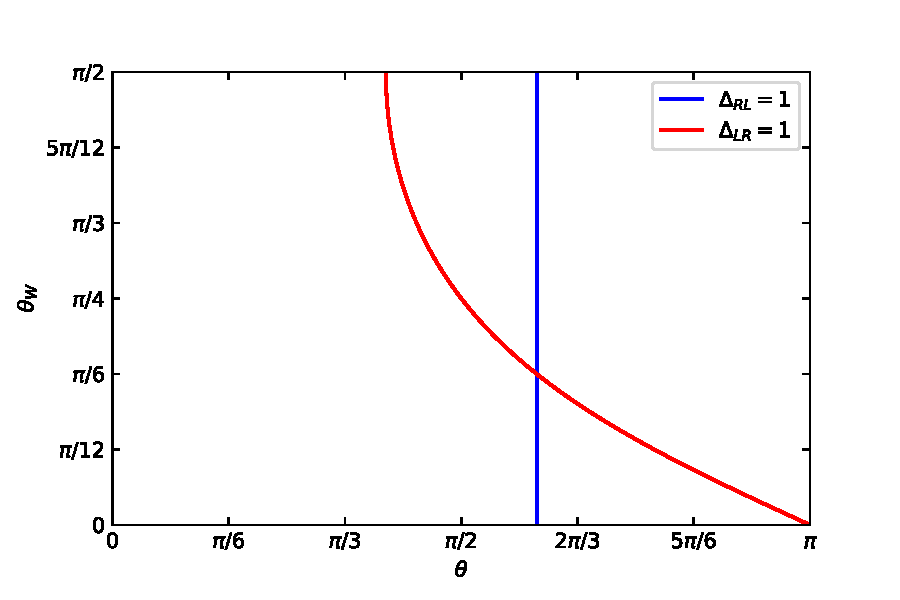
\includegraphics[width=0.85\linewidth]{concurrence.pdf}
		\caption{Líneas de máxima concurrencia para el ángulo de Weinberg \(\theta\) como función del ángulo \(\theta\) para el proceso \(e^-e^+\rightarrow\mu^-\mu^+\) incluyendo los efectos de la interferencia \(Z/\gamma\).} 
	\end{figure}
	
	\section{Conclusiones}
	En este trabajo hemos comprobado que imponiendo un principio de máxima entropía a las interacciones débiles obtenemos un valor para el ángulo de Weinberg similar al obtenido experimentalmente \(\theta_W = \pi / 6 \).  Este resultado positivo sugiere explorar que restricciones impondría la aplicación del principio de máxima entropía a las interacciones entre partículas, por ejemplo en QED, a todos los ordenes de aproximación.

	\bibliography{references}{}
	\bibliographystyle{ieeetr}	
\end{document}


